%% Use short name MACS MIS, CIMET, MTDMT, and if you are doing MMT or MIS  the language,  english or norwegian
\documentclass[MACS,english,a4paper,oneside]{ntnuthesis/ntnuthesis}

\usepackage[T1]{fontenc}
\usepackage[utf8]{inputenc}     % For utf8 encoded .tex files allows norwegian characters in the files. This can be dangerous if you change to a differnt editor.
\usepackage[pdftex]{graphicx, hyperref}   % For cross references in pdf
\usepackage{color}              % For colouring text 
\hypersetup{colorlinks=true,     
	linkcolor=blue,          % color of internal links (change box color with linkbordercolor)
	citecolor=blue,        % color of links to bibliography
	filecolor=blue,      % color of file links
	urlcolor=blue           % color of external links
}
\usepackage{csvsimple}  % for simple table reading and display
\usepackage{url}

%% added by me
	\usepackage{listings}
	\usepackage{tikz}
	%% include path for figures, graphics, etc
	\graphicspath{ {../figures/} }
	%% use tikz library for figures, nodes, images, etc.
	\usetikzlibrary{shapes.geometric,arrows}
	%% valid extensions for import in figures, etc.
	\DeclareGraphicsExtensions{.pdf,.png,.jpg,.jpeg,.bmp}
	%% to be able to comment out larger sections of text
	\usepackage{verbatim}
	
	% acronyms, abbreviations, etc.
	\usepackage[section,numberedsection=autolabel,acronym]{glossaries}
	\usepackage{makeidx}
	
	% Generate the glossary; must be called after hyperref
	\makeindex
	\makeglossaries
		
	%% Glossary/acronym list

%% example of how to add new acronym:
% \newacronym{gpu}{GPU}{Graphics}

%% 	A
\newacronym{ai}{AI}{Artificial~Intelligence}
\newacronym{aiml}{AIML}{Artificial~Intelligent~Markup~Language}

%% 	B
\newacronym{bn}{Bayes~Net}{Bayesian~network}
\newacronym{bow}{BOW}{Bag~of~Words}

%% 	C
\newacronym{ci}{CI}{Computational~Intelligence}

%% D
\newacronym{dag}{DAG}{Direct~Acyclic~Graph}

%% E

%% F

%% G
\newacronym{ntnu}{NTNU}{Norwegian University of Science and Technology}
\newacronym{nltk}{NLTK}{Natural Language Toolkit}

%% H
\newacronym{hmm}{HMM}{Hidden~Markov~Model}

%% I
\newacronym{ie}{IE}{Information~Extraction}
\newacronym{ir}{IR}{Information~Retrieval}
\newacronym{ia}{IA}{Intelligent~Agents}
\newacronym{ide}{IDE}{Integrated~Development~Environment}
\newacronym{its}{ITS}{Intelligent~Tutoring~System}

%% J

%% K

%% L
\newacronym{lms}{LMS}{Learning~Management~System}

%% M
\newacronym{ml}{ML}{Machine~Learning}

%% N

%% O

%% P
\newacronym{pos}{POS}{Part~of~Speech}
\newacronym{pr}{PR}{Pattern~Recognition}

%% Q
\newacronym{qa}{QA}{Question-Answering}
\newacronym{qc}{QC}{Question~Classification}

%% R

%% S
\newacronym{se}{SE}{Stack~Exchange}
\newacronym{so}{SO}{Stack~Overflow}
\newacronym{svm}{SVM}{Support~Vector~Machines}
\newacronym{svc}{SVC}{Support~Vector~Classification}
\newacronym{sgd}{SGD}{Stochastic~Gradient~Descent}
   


%% T

%% U

%% V

%% W

%% X

%% Y

%% Z



\begin{document}
	
	\setthesistitle{Question analysis of coding questions on StackOverflow}
\setthesisauthor{130533 - Knut Lucas Andersen}
\setthesissupervisor{Assoc. Prof. Simon McCallum}
%\setthesissupervisorA{Prof. Jon Yngve Hardeberg}  % if you have a second supervisor add it like this

\setthesisHostInstitution{\NTNU}
%\setthesisHostInstitution{University of Eastern Finland}
%\setthesisHostInstitution{Universit\'e Jean Monnet Saint-Etienne}

%\setthesisjuryA{} %jury names
%\setthesisjuryB{} %jury names
%\setthesisjuryC{} %jury names
%\setthesisjuryD{} %jury names

\nmtkeywords{Question-answering, Artificial Intelligence, scikit-learn, Question-analysis, Programming}
%\nmtdesc{This is the short description of a masters thesis}


\setthesisdate{31-05-2016}
\setthesisyear{2016}
%\setthesiscampus{Gj\o{}vik}
 % this is the file which contains all the details about your thesis
	\makefrontpages % make the frontpages
	
	%this is the intro to the thesis
%\thesistitlepage % make the ordinary titlepage
\hypersetup{pageanchor=false}
%\include{summary}

% \addcontentsline{toc}{chapter}{Preface}
\chapter*{Preface}
This is my Master thesis concluding the two years spent at NTNU Gjøvik: Master Applied Computer Science - Web, Mobile, Games track. 
The thesis was carried out during the spring semester 2016, from January to the end of May. 

The main concept for the thesis was based on discussions with supervisor. The original plan was to create a Chat Agent that could answers students questions and give feedback 
to their question quality, by using Stack Overflow as a knowledge base. However, during the Master thesis project presentation, other professors noted that the scope of the 
project was to large for a Master thesis. The thesis were therefore narrowed down to focus on coding questions posted on Stack Overflow, in an attempt to evaluate question quality 
and predict whether or not it was a good programming question. 

%\begin{center}
%\thesiscampus, 
\thesisdate \\[1pc]
\\[1pc]
%\thesisauthor
%\end{center}

% \addcontentsline{toc}{chapter}{Acknowledgment}
\chapter*{Acknowledgment}
I would like to thank the following persons for their help and support during these years. It would not have been possible without them.

My supervisor, Simon McCallum, for understanding my difficult situation and for his patience and helpful advices on how to proceed so that I could complete my Master thesis.

Mariusz Nowostawski for his advice on how to get started with text processing and ideas for building the SVM model. 

Rune Hjelsvold for helpful advice in relation to text analysis.

My best friend, Njål Dolonen, for always being there for me, and helped me get through this.

My grandmother, Mimmi H. Underland, may she rest in peace. None of this would have been possible without your support, understanding, love and care. This is for you.

I would also thank my family and friends for believing in me and supporting me through this.

\begin{flushright}
K.L.A
\end{flushright}
% reset glossary
\glsresetall
% \addcontentsline{toc}{chapter}{Abstract}
\chapter*{Abstract}
\gls{so} is today for many developers a well known \gls{qa} system. 
However, \gls{so} has a high requirement to the questions and answers posted, which is reflected through their voting and reputation system. 
This peer-review processes can be used as an indicator to a questions quality, where questions with high up-votes can be defined as good questions.
In this thesis, a system has been developed using  \gls{ml} and \gls{svm} to see if it is possible to predict whether or not a new question will be 
considered as a good or bad question. 
\vspace{0.5em}\newline
This was achieved by using the \gls{se} data set, specifically using the one for \gls{so}. 
Questions were dived into two classes, where bad questions was question with a vote score below zero, and good questions were those above zero. 
Based on content in the various questions, a set of feature detectors was developed and tested against the raw data set. 
Surprisingly, the features actually lowered the accuracy score.
The raw, unprocessed classifier achieved a score of 79.90\%.
The classifier using Porter stemming and all features achieved a score of 75.97\%, and the classifier without stemming using all the features got a score of 79.12\%.


\begin{comment}

- Peer-review process \\
- Duplicates \\
- Bias \\
- Code examples (or lack thereof) \\
- Easier to spot bad questions \\
- Homework is not accepted \\



%This is a summary of the thesis including the conclusion of what was discovered.

% write messy notes now, cleanup afterwards; ignore if its too much in this round..

When you have a question you need an answer to, the solution many uses is to go online and use Google or another  type of search engine. 
However, the degree of difficulty in regards to finding an answer varies with the problem you need an answer to. 
Today, the Internet offers a wide range of resources to acquire new knowledge, everything from encyclopaedias to blogs, forums and Question-Answer communities. 
However, when you are writing code, or developing complex programs, it can be easy to get stuck and not figure out why something stopped working. 
\vspace{0.5em}\newline
Depending on the complexity of the problem, the only solution might be to go to an online community for help. 
One such community is StackExchange (consisting of 154 different communities), which is home to StackOverflow. 
A requirement for all StackExchange sites is that questions should be of good quality. The quality of a question is measured by use of votes and reputation. 
The votes are used to grade the question (or answer), whereas the reputation belongs to the user. 
\vspace{0.5em}\newline
% Re-write paragraph below later on
By using \gls{ml}, I wanted to see if it was possible to predict whether a new question would be viewed as a goodquestion on StackOverflow. 
This was done by using the dataset containing all posts on StackOverflow and the \gls{ml} method \gls{svm} (by using scikit-learn for Python). 
A lot of time was used understanding how scikit-learn worked and how to properly implement \gls{svm} to analyse the questions. 
\vspace{0.5em}\newline
One of the interesting finds was that the average down-vote score for 10,000 was -7. 
To develop the feature detectors, a total of 100 good and bad questions were looked at to see if there was anything that stood out. 
It was a lot harder to find anything significant for what was a good question, but it was easier to spot the bad questions 
(e.g. homework, no code-samples, no explanation to what had been done before, etc.).
\vspace{0.5em}\newline
% double check numbers later on to see that these are indeed correct Before any processing was done, the \gls{svm} had a vocabulary of 69,766 features. 
To reduce this amount, stop-words were added (reducing to 69,462 features) and removal of numbers and hexa-decimal values (27,624). 
The most significant change was when the document term frequency were set to 1\%, which gave a total of 440 features.

Write something more about feature detectors, results, etc. \\
Note! Not actual abstract, more of a general introduction to later narrow down to abstract

\end{comment}

\hypersetup{pageanchor=false}
% reset glossary
\glsresetall
	
	\tableofcontents
	
	\hypersetup{pageanchor=true}
	
	% Comment with a percent to remove figures or tables:
	\listoffigures
	\listoftables
	
	
	%% Chapter list
	\chapter{Introduction}
	%\chapter{Introduction}
\label{chap:introduction}

Today, many uses the Internet as a resource to find answers to their questions and problems. 
In the past, one were often restricted to only use keywords and not being able to pose the problem as you would when asking another human being. 
Most search engines today can handle natural language queries, which makes it easier to find the answer you are looking for. 
The Internet offers a wide range of resources to acquire new knowledge, everything from encyclopaedias to blogs, forums and \gls{qa} communities.
One well known \gls{qa} community is the \gls{se} community, which is built upon the same model as \gls{so}.
\gls{se} has grown large since its release in 2009\todo[size=\small]{check year/ \\ date}, and now contains 154 different communities.
\vspace{0.5em}\newline
As a developer, one often find oneself in the situation that a part of the code does not work, you get weird error messages, or you are simply stuck. 
This is were \gls{so} comes in. \gls{so} is a part of the \gls{se} community, although \gls{so} was actually released before \gls{se}. 
Jeff Atwood and Joel Spolsky wanted to offer programmers a \gls{qa} site where they could get the answer they wanted without having to read through a lot of text, 
see others posting "I also have the same issue" or having to subscribe and pay to see the solution \cite{Spolsky2008}. 
Question (and answer) quality is maintained through the use of a peer-reviewed gamification system, where users are awarded with votes, reputation and badges for their 
participation\todo[size=\small]{add cites here} \cite{Spolsky2008}. One of the requirements is that the questions should be of good quality 
\cite{Stackoverflow.com2016a, Stackoverflow.com2016d, Stackoverflow.com2016e}.
If a question is bad, users can vote to close or delete it (in which the question will be put on hold). 
A question can be put on hold or closed if they meet any of the following criterias: 
Exact duplicate (same question has been asked before), off-topic (not related to \gls{so}), unclear what is being asked, too broad (e.g. could write a book about question being asked) 
or primarily opinion-based \cite{Stackoverflow.com2016b, CommunityWiki2016b}.


\begin{comment}

StackOverflow is a part of the StackExchange community, where each community is related to a specific field with domain experts. H
owever, a requirement is that the questions are of good quality \cite{Stackoverflow.com2016a, Stackoverflow.com2016d, Stackoverflow.com2016e}. 
Through peer-review, the quality of questions are filtered by using votes. If a question is good, it gets up-voted, if it is bad, it gets down-voted. 
The votes is only for the current question, but they still have an impact on the user, by use of reputation \cite{Stackoverflow.com2016c}. 
If a question is bad, it can be closed or deleted (e.g. duplicate, off topic, unclear, etc) \cite{Stackoverflow.com2016b}. 
\vspace{0.5em}\newline
The goal of this thesis is to research and analyse coding questions posted on StackOverflow. Most systems focus on finding good answers for the question asked, and not if it is a good question. 
It would therefore be interesting to see if it was possible to develop a system that could predict the quality of a question before posting it on StackOverflow.

When you have a question you need an answer to, the solution many uses is to go online and use Google or another  type of search engine. 
However, the degree of difficulty in regards to finding an answer varies with the problem you need an answer to. 
Today, the Internet offers a wide range of resources to acquire new knowledge, everything from encyclopaedias to blogs, forums and Question-Answer communities. 
However, when you are writing code, or developing complex programs, it can be easy to get stuck and not figure out why something stopped working. 
\vspace{0.5em}\newline
Depending on the complexity of the problem, the only solution might be to go to an online community for help. 
One such community is StackExchange (consisting of 154 different communities), which is home to StackOverflow. 
A requirement for all StackExchange sites is that questions should be of good quality. The quality of a question is measured by use of votes and reputation. 
The votes are used to grade the question (or answer), whereas the reputation belongs to the user. 
\vspace{0.5em}\newline
% Re-write paragraph below later on
By using \gls{ml}, I wanted to see if it was possible to predict whether a new question would be viewed as a good question on StackOverflow. 
This was done by using the dataset containing all posts on StackOverflow and the \gls{ml} method \gls{svm} (by using scikit-learn for Python). 
A lot of time was used understanding how scikit-learn worked and how to properly implement \gls{svm} to analyse the questions. 
\vspace{0.5em}\newline
One of the interesting finds was that the average down-vote score for 10,000 was -7. 
To develop the feature detectors, a total of 100 good and bad questions were looked at to see if there was anything that stood out. 
It was a lot harder to find anything significant for what was a good question, but it was easier to spot the bad questions 
(e.g. homework, no code-samples, no explanation to what had been done before, etc.).
\vspace{0.5em}\newline
% double check numbers later on to see that these are indeed correct
Before any processing was done, the \gls{svm} had a vocabulary of 69,766 features. 
To reduce this amount, stop-words were added (reducing to 69,462 features) and removal of numbers and hexa-decimal values (27,624). 
The most significant change was when the document term frequency were set to 1\%, which gave a total of 440 features.
\end{comment}


\section{Problem description}
\label{sec:problem_description}
Most of the systems that have been developed so far\todo[size=\small]{add examples here}~focuses on finding the best answer to a question asked by the user. 
Few, if any, focuses on the quality of the question being asked. 
What defines a good question, and can we in anyway predict whether or not a new question posted on \gls{so} will be considered good or bad by the community?
There are many users who has either a negative view or relationship in regards to \gls{so}.
Many experience that their questions gets down-voted, closed or even deleted. 
For some, they simply do not know how to ask an acceptable question.
Questions related to homework are one example of questions that are not accepted on \gls{so}.
There is even a post on Meta.StackExchange discussing whether or not it should be acceptable to use greetings and sentiments in posts\cite{CommunityWiki2016a}.
Therefore, the question becomes: What is and is not a valid question on \gls{so}?
%What if there was a system that could give a prediction on the quality of your question?

\section{Research questions}
\label{sec:research_questions}

\begin{itemize}
	\item What defines a good (coding) question on \gls{so}?
	\item Can we predict a questions quality by using \gls{svm}?
	\item What type of features increases the accuracy of the \gls{svm}?
\end{itemize}

\section{Methodology to be used}
\label{sec:methodology_to_use}
The theoretical background in this thesis is mainly focused on \gls{qc} and similar research in relation to \gls{so}.
What has been the focus of other researchers, and in what way did they proceed to solve their questions?
The analysis of the questions are done by using the publicly available database dump, which is available via \gls{se} 
archive\footnote{StackExchange dataset: \url{https://archive.org/details/stackexchange} \\ (Downloaded 30. March 2016).} \cite{StackExchange2016} . 
There are several others who have used the same dataset \todo[size=\small]{add cites here}.
Taking into consideration that \gls{so} was released in 2008, it means that it now contains approximately 8 years of peer-revied data.
Because of the size of the data set, and the total amount of posted questions, going through all questions manually would be too timeconsuming.
Therefore only a select few were studied too see if it was possible to identify what separated the highly up and down-voted questions.
\vspace{0.5em}\newline
The goal was to develop a \gls{ml} learning system which was based on \gls{svm}, since many papers document that this has the best classification accuracy for text classification. 
The methodology therefore also includes a documentation on the development process, and how and why the given features used were selected.
\vspace{0.5em}\newline
For the sake of replicability, and also be able to undo potential errors, the system is available in a a GitHub repository\footnote{
	GitHub repository: 
	\url{https://github.com/klAndersen/IMT4904_MasterThesis_Code}
}. 
In addition to the source code, the repository also contains both the samples that was used (stored in CSV files), and the models that was created. 

% \todo[size=\small]{add cites here}~

\section{Justification, Motivation and Benefits}
\label{sec:justification}
Many systems focuses only on finding a good answer, and does not ask if it is a good question.
As a famous Norwegian saying goes\footnote{
	Although its origin comes from a Danish word collection from 1682: 
	\url{https://snl.no/En\_d\%C3\%A5re_kan_sp\%C3\%B8rre_mer_enn_ti_vise_kan_svare}.
}: "A fool may ask more than ten wise men can answer".
This means that new research possibilities could be opened up in relation to researching question quality by expanding the system. 
Since all the communities within \gls{se} is based on the same model, few modifications would be needed to scale the program to be used within the other communities.
As noted in several papers\todo[size=\small]{add cites here}~, question quality is measured based on the amount of votes given. 
Which can also be compared against the peer-review process in academia, and given that \gls{so} targets professionals and experts, 
using \gls{so} as a scientific reference is not that far-fetched (in CITE, XX\% used \gls{so} as a reference). 
\gls{se} has also been the focus of various researchers these past years \cite{Vasilescu2012}.
Improving ones own ability to ask better questions can also have a pedagogical effect, which means that this system could be implemented in education. 

\begin{comment}
The quality of a question is based on the votes given by the users of the StackOverflow community. 
Therefore the vote score was used to label the question as either good (score > 0) or bad (score < 0). 
This is justified by the fact that you can draw a comparison between the peer-review process used in academia and the peer-review process used in StackOverflow. 
The process starts with someone posting a question, which is then read, scored and given feedback (through comments or answers). 
The feedback can then improve the question through edits by the poster, based on the feedback given 
(e.g. adding additional information or explaining how the given problem(s) occurred).
\vspace{0.5em}\newline
Scikit-learns \gls{svm} implementation is based on libsvm \cite{ChangLin2011}, but it is simpler to use. 
In addition, scikit-learn focuses on code quality\footnote{Coverage on their GitHub repository was 94\% on 06. May 2015.}, 
to ensure that everything works as it should \cite[p.~3]{PedregosaVaroquauxGramfortEtAl2011}.
\vspace{0.5em}\newline
It is not a lot of research being done related to asking and defining good questions. 
Although the focus is only on programming questions, it can still be useful to improve question quality. 
Even if you cannot predict if it is a good question, you can still avoid asking a bad questions. 
This in turn can help to improve the question quality (at least acceptability), and avoid asking questions that will be closed or ignored on StackOverflow.
\end{comment}

\section{Limitations}
\label{sec:limitations}
The greatest limitation is the time available. 
A large amount of time was spent on setting up the database, and retrieving the questions (the Posts table contains both questions and answers).
Only a selection of the questions were selected (a total of 20,000 questions), and training the \gls{svm} over one sample set can easily take several hours. 
This also has an impact on classification accuracy, since in some cases there is only a small amount of the questions that contains a given feature 
(e.g. the hexadecimal feature, which only was present in 160/20,000 questions).
A limitation is also that the focus is only on \gls{so}, which means that one would need to make additional adjustments and add more filtering to account 
for the differences that may occur in each community.
 
\section{Thesis contribution}
\label{sec:thesis_contribution}
This thesis contribution can be summarized as to the following: 
Predicting (programming) question quality by  using \gls{ai} and \gls{ml} to improve the questions quality. 
Instead of posting bad questions that can get down-voted or closed, the developed system could be able to give feedback to the questions quality. 
Furthermore, the research presented could open up for new research in relation to how we ask questions online, and in what ways these best can be analysed.
It can also be used for educational purposes, e.g. having questions iteratively improve their question quality by asking the system questions.

\section{Thesis structure}
\label{sec:thesis_structure}
The following is the structure of this thesis:
\begin{itemize}
	\item Chapter \ref{chap:chapter2}: State of the art and relevant research
	\item Chapter \ref{chap:chapter3}: Methodology 
	\item Chapter \ref{chap:chapter5}: Discussion on development, the thesis and limitations
	\item Chapter \ref{chap:chapter6}: Conclusion and suggestions for further work
\end{itemize}
 
	
	\chapter{Related work}
	%\chapter{State of the art}
\label{chap:chapter2}

\section[Stack Overflow]{\glsentrylong{so} (\glsentryshort{so})}
\label{sec:stackoverflow}

\subsection[Stack Overflows design]{\glsentrylong{so}s (\glsentryshort{so}) Design}
\label{sec:stackoverflow_design}
The following list shows the design used in \gls{so} (based on \textcite[p.~6-7]{M.Sewak2010} and \textcite[p.~805]{Treude2011}):
\begin{enumerate}
	\item Votes: Questions and answers which are considered good (or bad) by the community can be given a score. 
	This gives a filtering mechanisms, which allows users to ignore answers that are bad or wrong. 
	Furthermore, answers are sorted by votes, and you can also sort questions on \gls{so} by vote score 
	(see Figure \ref{fig:question_list_acc_answ}). 
	\item Accepted answer: If the user asking a question gets an answer that they find satisfactory, they can select it as the "accepted answer". 
	This answer will be the first displayed of the answers, and is also viewable when searching for questions 
	(see Figure \ref{fig:question_list_acc_answ} and \ref{fig:so_question_example}).
	\item Tags: Each question is associated with a tag\footnote{
		A full list can be seen here: \url{http://stackoverflow.com/tags/}
	}, which can be a topic, a programming language, a methodology, etc.
	\item Badges: Similar to achievements in games, Badges are used to reward the user for their participation.
	\item Reputation and Bounty: Currency system for user participation. 
	E.g. voting for questions, getting your answer selected as the accepted one, etc.
	Bounty is a trade, where if your question goes unanswered for too long, you offer up parts of your reputation to receive an answer.
	\item Data dump: Available data dump containing all content available within the \gls{se} community \cite{StackExchange2016}. 
	You can either download single files, or everything by using a Torrent client.
	\item Pre-Search: Encouraging users to check that their question is not already posted by presenting a search bar when asking a new question. 
	\item URL keywords and Google: The questions title is included in the URL, allowing it to be processed by search engines. 
	In addition, Google uses their crawlers every 10 second to have the latest updates from \glossary{so} in their search engine \cite{Gobry2011}.
	\item Critical mass: Before Atwood and Spoolsky launched \gls{so}, they invited developers and programmers to participate to have some domain experts available. 
\end{enumerate}

\clearpage
% figure showing questions, where one question has an accepted answer
\begin{figure}[ht]
	\centering
	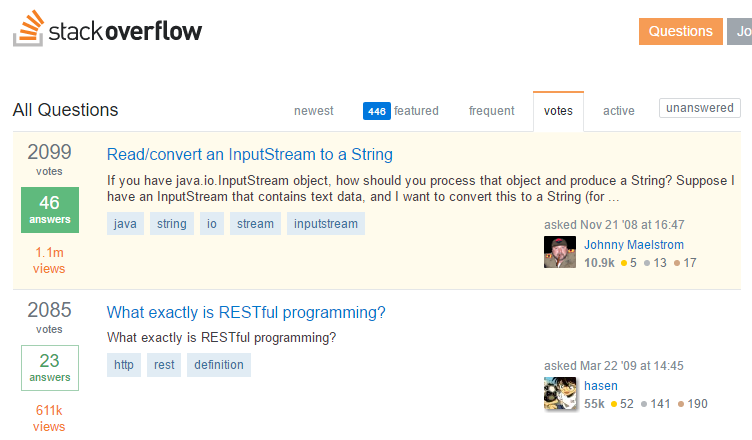
\includegraphics[width=0.5\textwidth]{question_list_acc_answ}
	\caption{List of questions, where one can see those with an accepted answers are marked with a green background.}
	\label{fig:question_list_acc_answ}
\end{figure}


% figure showing page with question and answer
\begin{figure}[ht]
	\centering
	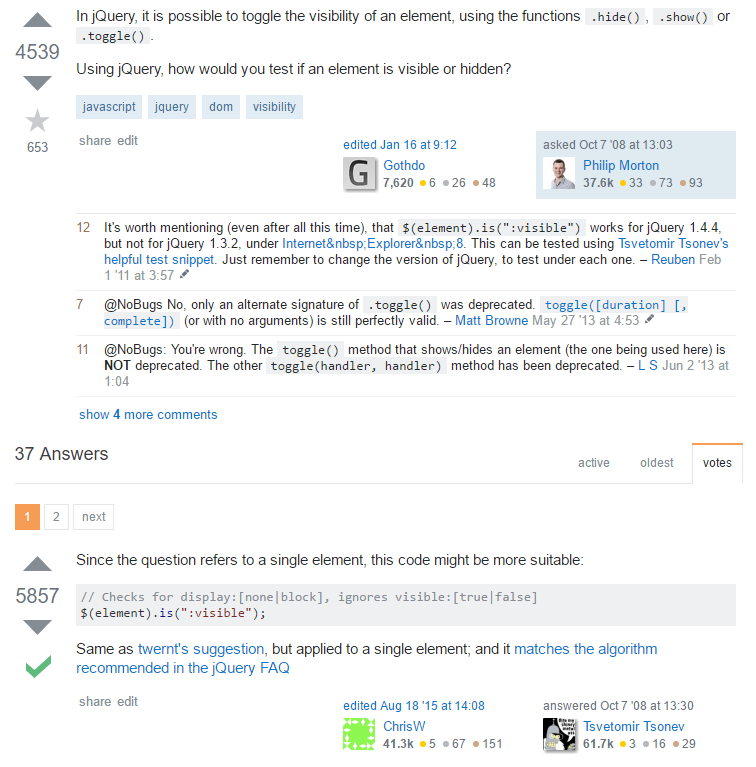
\includegraphics[width=0.5\textwidth]{so_question_example}
	\caption[Example of a question on Stack Overflow]{Example of a question on Stack Overflow\footnotemark}
	\label{fig:so_question_example}
\end{figure}
\footnotetext{Source: \url{http://stackoverflow.com/questions/178325/checking-if-an-element-is-hidden}}

\subsection[Stack Overflow and Gamification]{\glsentrylong{so} (\glsentryshort{so}) and Gamification}
\label{sec:stackoverflow_gamification}
\textcite{Deterding2011} defines Gamification as "the use of game design elements in non-game contexts", and is the definition this section will be based on. 
Several papers make notes of the pedagogical and educational aspect of \gls{so} \cite{Nasehi2012, Posnett2012, Yang2014}, and \cite{Nasehi2012, Yang2014} use the term gamification in their paper.
One of the founders, Jeff Atwood said in an interview that he wanted users to not just give good answers, but also trick them into improving their communication skills \cite{Posnett2012}\footnote{
	From this interview: \\ 
	\url{http://www.wired.com/2012/07/stackoverflow-jeff-atwood/2012}.
	}.
In the course IMT4007 Serious Games Simon McCallum and Marius Nowostawski, presented their game GoRad, which was based on us students reading articles and posting questions which were voted on. 
The \gls{so} system awards users based their activity by using votes, reputation and badges \cite{M.Sewak2010, Movshovitz-Attias2013, Treude2011, StackOverflow.com2016, StackOverflow.com2016d}.
In relation to gaming, there are four player types: Achievers, Explorers, Socializers and Killers \cite[p.~3]{Maan2013}.
\vspace{0.5em}\newline
These player types can be used as a representation\footnote{	
	\textcite{Yang2014} characterised users as "Sparrows" and "Owls", where sparrows answers question for reputation and owls answers the difficult ones (domain experts).  \\
	\textcite[p.~2]{Ahmed2015} defined users as "lurkers, help-seekers (askers) and givers (responders)".	
	} for the various users of \gls{so}. 
Achievers are there for the reputation and badges, socializers are to interact, discuss and share knowledge. 
Explorers might find joy in looking at various topics, or searching for unanswered questions.
The only exception would be the "Killer" type. 
Killers are those "\ldots who always want to create trouble/problems for other participants" \cite[p.~3]{Maan2013}. 
In an online \gls{qa} system (or Internet in general), these are what are commonly referred to as "Trolls" \cite{Fosdick2012, Atwood2015}. 
However, due to the system used in \gls{so}, Trolls would not be able to survive, simply because the reputation controls what you have access to \cite{StackOverflow.com2016g}. 
If you down-vote a post, you lose reputation. 
If your post gets down-voted, you also lose reputation. 
Users who are not willing to follow the guidelines can be locked out of \gls{so} \cite{Atwood2009}.
However, today there is a lot of blogs complaining about the current structure of \gls{so}, who claims that a lot of the moderators are
trolls\footnote{\url{https://www.reddit.com/r/programming/comments/3cafkp/is_stack_overflow_overrun_by_trolls/}. \\	
	\url{https://medium.com/@johnslegers/the-decline-of-stack-overflow-7cb69faa575d} \\ 
	Last accessed 23.05.2016. 
}.

\subsection[Stack Overflow and reputation]{\glsentrylong{so} (\glsentryshort{so}) and reputation}
\label{sec:research_on_so}

Many \gls{qa} sites includes domain experts to ensure some quality is upheld, and uses voting and reputation as a quality measurement \cite{Anderson2012}.
Furthermore, questions topics, page views and votes can be used by search engines as a ranking mechanism, and it helps users to find the answers they are looking for. 
\textcite{Anderson2012} identifies two principles for the answer process. 
This process starts with the question being filtered down through the users, starting with domain experts. 
If the domain experts does not answer, it goes further down the chain, until it in the end either gets an answer, or is not answered at all.
Both \textcite{Anderson2012} and \textcite{Treude2011} defines an unanswered question to be a question where no accepted answer is chosen\footnote{
	However, they do not take into considerations users who find a solution on their own, or simply forget or neglect to mark a an answer as accepted.
}. 
The second principle is that a questions activity level does not just indicate the interest for the question, but could also be an indicator for quality 
(because a question can have multiple answers). 
\vspace{0.5em}\newline
Since users can only gain 200 reputation points daily, the only way to earn more is by having your answer marked as accepted or through bounties \cite{StackOverflow.com2016d}.
\textcite{Movshovitz-Attias2013} found that users earn more reputation by providing good answers rather than good 
questions\footnote{
	However, as stated in \textcite[p.~3]{Movshovitz-Attias2013}, the reputation system was changed at one point. 
	Originally, up-votes on questions and answers gave users a +10, but this was later changed into up-votes on questions only giving +5. 
}.
Most questions was asked by the users with a low reputation, but on average users with high reputation asked more questions. 
This indicates that reputation could be used as a measurement for expertise. 
\textcite{Ahmed2015} also found that there was a correlation between amount of answers given and the users reputation.
\vspace{0.5em}\newline
\textcite{Yang2014} found that the activity level of a user is not equal to knowledge, and divided users into two groups; "Sparrows" and "Owls".
The sparrows are the basic users who earns reputation and badges by answering the easy questions, and has a greater interest in the gamification element. 
They found that the sparrows usually has a low average score and targets questions that are easy, or non-relevant. 
Nonetheless, they are still important since they are able to provide quick feedback.
As for the owls, they are considered to be the domain experts.
The owls earn reputation by asking more advanced questions, providing better answers (i.e. getting their answer accepted) and answering popular and difficult\footnote{
	Popularity was measured based on page views and the time between a question was posted until an answer was selected as accepted.
	The popularity can also therefore be seen as a measurement for difficulty.
	The longer it takes to answer, the more difficult the question is~\cite[p.~273]{Yang2014}.
} questions.
\vspace{0.5em}\newline
\textcite{Posnett2012} views \gls{se} and \gls{so} as a learning community, since users help each gain new knowledge, and motivates learning.
They wanted to see if the quality of the users answers improved over time. 
By constructing a posting history for each user, they found that the overall answer score decreased, and that the answer quality was static.
\vspace{0.5em}\newline
\textcite{Nasehi2012} did a qualitative analysis of code examples posted on \gls{so}. 
Their focus was on questions related to Java programming, with the requirements that the question should at least have a score of +4 and the answer +7. 
In addition, a code example should be included (by checking for <code> in the post).
They found that the code explanation was just as important as the code examples (but you are still restricted to the quality of that example).
For the code to be considered good, they listed the following attributes: 
\begin{enumerate}
	\item Concise code: Code samples should not be too long. 
	They should be simple, and only focus on the parts that are relevant to the topic.
	Additional or non-relevant parts should instead be documented by using descriptive comments.
	\item Question context: 
	If the code is not working properly, suggestions for improvement should be added. 
	One could also explain best practices and suggestions for improved readability.
	This will also have a pedagogical benefit, since the user asking the questions will learn to write better code.
	\item Highlighting important elements: 
	"Straight to the point", clearing up misunderstandings, pointing to relevant resources, etc.
	\item Step-by-step solution: 
	Splitting code into chunks, and explaining each chunk and its functionality.
	Comparison of languages; e.g. "How can I do X in C\#, when I'm used to Java?"
	\item Providing links to extra resources: 
	Answers can be kept short by adding links to external resources, but a short summary should still be added.
\end{enumerate}


\section{Asking questions}
\label{sec:asking_questions}

\subsection{What is the definition of a question?}
\label{sec:question_definition}
The context of a question varies within the setting it is used. 
A question can be broad, where multiple answers can all be correct, or they can be factual, having only one right answer. 
When you are asking someone a question, you ask because you want to either find a solution to a problem, or learn something new. 
In the context of learning, questions are used for evaluating the students knowledge, or help them learn something new \textcite{Nielsen2008}.
\vspace{0.5em}\newline
When doing research, you need research questions and hypotheses to decide what the goal of your research is. 
What questions are you trying to find an answer to, and what does that answer tell you?
\textcite{Slowiaczek1992} defines asking a question as information selection and the answer(s) to a question as information usage. 
If you are working with statistical data, and you just post the numbers, this will not inform anyone. 
You need to explain what the numbers mean, and how you got them.
The quality of an answer is also restricted to the quality of the question you ask. 
One can therefore assume that if you ask a good question, you will get a good answer \cite{Slowiaczek1992}. 

\subsection[Question classification]{\glsentrylong{qc} (\glsentryshort{qc})}
\label{sec:question_classification}
\gls{qc} is the process of categorizing a question into a class or category based on its structure, usually to decide what the expected answer type is \cite{Li, Loni2011, Lopez2011}. 
To classify a question, it is important to select only those features that helps you identify the class it belongs to.
To get a classification results, you use what is known as a classifier. 
The quality of a classifier can be measured by its accuracy and precision (see Equation \ref{eq:accuracy} and \ref{eq:accuracy}; taken from \cite[p.~13]{Li}).

\begin{equation}\label{eq:accuracy}
Accuracy = \frac{\#~of~correct~predictions}{\#~of~predictions}
\end{equation}

\begin{equation}\label{eq:precision}
Precison[c] = \frac{\#~of~correct~predictions~of~class~c}{\#~of~prediction~of~class~c}
\end{equation}

\paragraph{WH-words}
\label{sec:wh_words}
WH-words are mostly found in factoid questions \cite{Lopez2011}. 
\textcite{Huang2008} listed eight different WH-words: What, which, when, where, who, how, why, and rest (rest being the type does not belong to any of the previous type). 
\textcite{Letovsky1987} also listed "Whether" and "Discrepancy"\footnote{
	"Questions that reflect confusion over a perceived inconsistency." \cite[p.~5]{Letovsky1987}
}.
However, not all are equally easy to use for classification, because even if the questions ask for the same answer, wording and syntactic structures can make it difficult to classify.
Question containing words like "What", "Why", "How" and "Which", can be harder to classify due to the lack of limitation in regards to answer types\footnote{
	An answer type (or named entity) is the expected type of the answer to a given question (e.g. a Location, Organization, Person, Date, etc) \cite{Heie2012, Lopez2011, Sasaki2005, Yen2013}. 
} \cite{Huang2008, Lopez2011}.


\paragraph[Bag-of-words and N-grams]{\glsentrylong{bow} (\glsentryshort{bow}) and N-grams}
\label{sec:bow}
N-gram is a model that is used for splitting text into either characters (character model) or word frequencies (word model). 
The \gls{bow} model (or unigram) only looks at singular words, ignoring the order and relies only on the frequency for each word \cite{Manning2008, Russell2013}. 
Bi-grams takes dual values, tri-gram takes three, etc.
\vspace{0.5em}\newline
One problem with N-grams is that the dimension of the feature space is equal to the amount of words in the vocabulary \cite{Russell2013, Loni2011}
When using categorization, there can be issues with mapping new words that does not exist in the vocabulary \cite{Yen2013}.
The impact of N-gram is also related to the size of the text being analysed. 
\textcite{Zhang2003} found that there was not a big difference when using between bag-of-ngrams (all continuous word sequences in the question) and \gls{bow} as features.


\paragraph{Word mapping and processing: Case-sensitivity, Stemming, Stop words and Tokenization}
\label{sec:word_mapping_processing}
To reduce the amount of words used, there are more steps that can be taken. 
By removing the case-sensitivity, all words will be equal (e.g. is the word 'Hello' equal to the word 'hello'?).
\cite{Huang2008} includes case-sensitivity under a definition called word shape, consisting of five elements: upper case, all lower case, mixed case, all digits, and other.
\vspace{0.5em}\newline
Semantics can be used for word filtering, e.g. removal of duplicate words or words with same meaning. 
WordNet has a built in function called synsets() which removes synonyms (words having the same meaning). 
You can also look for hypernyms (words belonging to a category with a parent-child relationship) or use stemming.
Stemming reduces the word to its base-form, e.g. crying would be converted into the word cry.
Word separation is also possible through tokenization, which splits the text into an array based on a set delimiter.
There is also usage of stop words for removal of frequently used words in a given language.
\vspace{0.5em}\newline
%Stop words \cite{Manevitz2002, Wang2013, Zhang2003, Kaestner2013, Joachims1998}
Grammatical properties can be extracted by using \gls{pos}, e.g. by using \gls{nltk}\footnote{
	\gls{nltk} includes in their \gls{pos} tagger the following grammatical properties:
	Adjective, adposition, adverb, conjuction, determiner, article, noun, numeral, particle, pronoun, verb, 
	punctuation mark and others	 \cite[See Section 2.3]{StevenBird2015}.
}, which can be helpful in reducing ambiguities \cite{Bloehdorn2004}.
\textcite{Li} uses the word head chunks to identify what the question is asking for when multiple types are introduced (avoid ambiguity). 
The same concept is used in \cite{Huang2008} and \cite{Loni2011}, but there it is referred to as headwords.

\subsection{Text classification}
\label{sec:text_classification}
The goal of text classification (or text categorization) is to be able to process multiple documents or large amounts of text into categories. 
It shares similarities with question classification, although an obvious difference would be the size of the text that is processed. 
Some examples are spam filtering \cite{Russell2013, Kaestner2013}, to identify languages, or filing documents based on content \cite{Kaestner2013}.
Documents can belong in more then category, and since categories can overlap they must be treated as a binary classification problem \cite{Joachims1998} .
Text classification starts with retrieval of the documents, usually by using \gls{ir} methods, and then transforming the text into features for the classification. 
When you have a large amount of text, you can easily get a feature space that is very high dimensional, and that is why feature selection is important. 
Feature selection is the selection of features (or attributes) that are important for the classification. 
E.g. if you were classifying documents based on colour description, then hypernyms for colour would be an important feature.


\subsection[Question-Answering]{\glsentrylong{qa} (\glsentryshort{qa})}
\label{sec:question_answering}
\gls{qa} is mostly used as a method for finding the answer to a question from an unknown amount of documents.
When using a search engine, one can accept that there are several results that are listed because at least one of the search terms exists. 
However, when using a \gls{qa} system, users wants the answer straight away instead of having to read through several documents. 
In addition, \gls{qa} sites allows users to search for questions in the same way they would ask another human (natural language\footnote{
	However, there is a problem with linguistics in natural language systems \cite{Lopez2011}.
	}), 
and there are also different types of \gls{qa} sites.
Domain specific \gls{qa} focuses on a specific topic (e.g. \gls{so}) and open domain where everything goes. 
\gls{qa} sites can also function as an archive or a knowledge base, since all the posts are available even years after they were posted.
\vspace{0.5em}\newline
\textcite{Yen2013} found that it was more efficient searching for answers in a small dataset, then the document as a whole. 
By using a passage retriever, the documents were split into paragraphs and ranked by using evaluation metrics. 
\textcite{Isozaki2005} could not use TF-IDF based paragraph retrieval, because the paragraphs were too short to cover all query terms. 
If the terms that were used were too short or too long, the passage scores would not reflect the density distribution. 
\textcite{Xu2012} built an online \gls{qa} system for tourism, which consisted of question analysis, information retrieval and answer extraction.
Since rule-based approach requires expert knowledge, creating features that are domain specific can improve accuracy (what they called "domain term concept hierarchy").
To validate the classification, they tested the results by using 5-fold cross-validation.
\vspace{0.5em}\newline
\textcite{Li} used semantics to categorize questions based on the possible semantic answer type. 
One issue with questions are that since they can be very short, they contain little text. 
However, the lack of long text improves both the accuracy and analysis. 
\vspace{0.5em}\newline
\textcite{Zhang2003} says that \gls{qc} is important, and simply looking for WH-words is not enough. 
By using WH-words, headwords, WordNet semantics, N-grams and word shapes as features, and a linear \gls{svm} and Maximum Entropy model, 
they reached an 89.2\% and 89.0\% over a standard benchmark dataset. 
They also experimented with four other algorithms, Nearest Neighbours (simplified version of k-NN),  Naive Bayes and Decision Tree and Sparse Network of Winnows (SNoW).
However, these were outperformed by the \gls{svm}.


\section[SVM]{\glsentrylong{svm} (\glsentryshort{svm})}
\label{sec:svm}

\gls{svm}s are good for solving regression and classification problems, and attempts to solve a linearly separable problem by using hyperplanes \cite{Duda2001, Kononenko2007, Russell2013}.
It is usually used for binary classifications, where classes are represented as either +1 or -1 \cite{Manning2008, Russell2013}. 
The hyperplane is the plane which separates the two classes: 
% hyperplane equation
\begin{equation}\label{eq:hyperplane}
\vec{w}^{T}\vec{x} = \textit{-b} 
\end{equation}
where \textit{b} is the intercept term and $\vec{w}$ is the weight vector (or decision hyperplane normal vector).
The data set can be represented as $\mathbb{D} = \{(\vec{x}_{i}, y_{i})\}$ where $\vec{x}_{i}$ is a data point, and $ y_{i}$ is its belonging class label.
The linear classifier is represented in Equation \ref{eq:linear_classifier}  \cite[p.~295-296]{Manning2008}. 
% linear classifier
\begin{equation}\label{eq:linear_classifier}
f(\vec{x}) = sign(\vec{w}^{T}\vec{x} + b)
\end{equation}
% space
In addition to using a hyperplane, the \gls{svm} has an additional separation known as support vectors. 
Support vectors are the training points closest to the margin (the margin is the distance from the hyperplane) \cite{Duda2001, Manning2008}.
Which then gives that the optimal hyperplane is the furthest from the support vectors \cite{Kononenko2007}.
% space
\gls{svm} has four different kernels, but a limitation is that there is no way to select the best kernel function. 
Therefore, \gls{svm} often uses hyper-parameters and select the classifier based on the best results \cite{Theodoridis2009}.
Equation \ref{eq:kernel_polynomial} - \ref{eq:kernel_sigmoid} shows the kernel functions (K) for polynomial, radial basis function (RBF) and sigmoid (taken from \cite[p.~273]{Kononenko2007}). \\
% polynomial kernel
Polynomial - for a given polynomial degree \textit{d}, the following is used:
\begin{equation}\label{eq:kernel_polynomial}
K (\textbf{x}_{j}, \textbf{x}) = [(\textbf{x}  \cdot \textbf{x}_{j}) + 1]^{d}
\end{equation}
% rbf kernel
Radial - for a given $\gamma$ value, the following is used:
\begin{equation}\label{eq:kernel_rbf}
K (\textbf{x}_{j}, \textbf{x}) = e^{-\gamma|\textbf{x}-\textbf{x}_{j}|^{2}}
\end{equation}
% sigmoid kernel
Sigmoid - for a given sigmoid function S, we get a kernel function of parameters \textit{v} and \textit{c}: 
\begin{equation}\label{eq:kernel_sigmoid}
K (\textbf{x}_{j}, \textbf{x}) = S(\textit{v}(\textbf{x}  \cdot \textbf{x}_{j}) + c)
\end{equation}

For text classification, in most cases it will be non-linearly separable. 
One can therefore allow the \gls{svm} to do some mistakes.
However, there is a cost for misclassifications, represented by what is called a slack variable $\xi_{i}$.
If $\xi_{i}$ is set (not zero), then the vector can miss the margin requirement at the cost of $\xi_{i}$.
Equations are shown in Equation \ref{eq:slack_variable1} - \ref{eq:slack_variable3} (taken from \cite[p.~301]{Manning2008}). \\
Find
% slack variable optimization - 1
\begin{equation}\label{eq:slack_variable1}
\vec{w}, b~and~\xi_{i} \geq 0
\end{equation}
% slack variable optimization - 2
so that we can minimize the optimization problem
\begin{equation}\label{eq:slack_variable2}
\frac{1}{2}\vec{w}^{T}\vec{w}~+~C\sum_{i}\xi_{i}
\end{equation}
% slack variable optimization - 3
and for all
\begin{equation}\label{eq:slack_variable3}
\{(x_{i}, y_{i})\},~y_{i}(\vec{w}^{T}\vec{x}~+~b) \geq 1 - \xi_{i}
\end{equation}
However, this gives a trade-off between the size of the margin and how much the data points can be adjusted. 
To avoid overfitting, the parameter C is used for regularization, where the size of C decides how much flexibility you get from the slack variable \cite{Manning2008}.
\gls{svm} neither suffer from the Curse of dimensionality, because the computational complexity is independent of the kernels dimensional space~\cite{Theodoridis2009}.


% SHOULD THIS BE USED?
%\gls{svm} uses the maximum margin solution, which is based on computational learning theory\footnote{	
%	Computational learning theory is an attempt to understand how large a data set needs to be in order to give good generalization \cite[p.~344]{Bishop2006}.
%} \cite{Bishop2006, Joachims1998}.
%
%
%
%% keep this sentence; its properly re-written
%For \gls{qc} a question is usually represented as a vector space model, where each vector contains the words from the question \cite{Loni2011}.

\textcite{Joachims1998} found that \gls{svm} consistently achieved good performance during text categorization. 
Since \gls{svm} could generalize in high dimensional feature space, the need for feature selection was removed, and \gls{svm} was also robust. 
Since \gls{svm} does not require parameter tuning, they could find good parameter settings automatically. 
\textcite{Loni2011} found that \gls{svm} are successful on high dimensional data when it is sparse, but they still suffer from redundant features. 

\begin{comment}
% Re-write and use what ever fits
\gls{svm}s
are very successful on high dimensional data since they are
timely efficient especially when the feature vectors are sparse,
but they still suffer from the redundant features.
\gls{svm} is a linear discriminant model which tries to find a
hyperplane with maximum margin for separating the classes.
They are fast classifiers for high dimensional data [13]. To
be able to linearly separate data, the feature space usually is
mapped to a higher dimensional space. The mapping is done
with a so-called kernel function. The most widely used kernel
in question classification is the linear kernel. 
\cite{Loni2011}


\gls{svm} is based on the Structural Risk Minimization principle from computational learning theory. 
The idea of structural risk minimization is to find a hypothesis h for which we can guarantee the lowest true error.  
The true error of h is the probability that h will make an error on an unseen and randomly selected test example. 
An upper bound can be used to connect the true error of a hypothesis h with the error of h on the training set and the complexity of H (measured by VC-Dimension), the hypothesis space containing h. 
\gls{svm}s find the hypothesis h which (approximately) minimizes this bound on the true error by effectively and efficiently controlling the VC-Dimension of H.
One remarkable property of \gls{svm}s is that their ability to learn can be independent of the dimensionality of the feature space. 
\gls{svm}s measure the complexity of hypotheses based on the margin with which they separate the data, not the number of features. 
This means that we can generalize even in the presence of very many features, if our data is separable with a wide margin using functions from the hypothesis space. 
The same margin argument also suggest a heuristic for selecting good parameter settings for the learner (like the kernel width in all RBF network). 
The best parameter setting is the one which produces the hypothesis with the lowest VC-Dimension.
This allows fully automatic parameter tuning without expensive cross-validation. \\
Theoretical analysis concludes that \gls{svm}s acknowledge the particular properties of text: 
\begin{itemize}
\item high dimensional feature spaces, 
\item few irrelevant features (dense concept vector), 
\item sparse instance vectors.
\end{itemize}
Experimental results show that \gls{svm}s consistently achieve good performance on text categorization tasks, outperforming existing methods substantially and significantly. 
With their ability to generalize well in high dimensional feature spaces, \gls{svm}s eliminate the need for feature selection, making the application of text categorization considerably easier.
Another advantage of \gls{svm}s over the conventional methods is their robustness. 
\gls{svm}s show good performance in all experiments, avoiding catastrophic failure, as observed with the conventional methods on some tasks. 
Furthermore, \gls{svm}s do not require any parameter tuning, since they can find good parameter settings automatically. 
All this makes \gls{svm}s a very promising and easy-to-use method for learning text classifiers from examples.
\cite{Joachims1998}
\end{comment}


\section{Dataset}
\label{sec:dataset}
short about the datasets, others who has used it, and datasets in general, e.g. 
\cite{Klein2016,SpaceMachine.net2016,Wissner-Gross2016}









\section{undefined}
\label{sec:undefined}
% stuff everything that doesn't fit elswhere bu is still of relevance

\textcite{Stanley2013} - Predicting Tags for StackOverflow Posts

\textcite{Short2014} - Tag Recommendations in StackOverflow

\textcite{Wang2013} - An Empirical Study on Developer Interactions in StackOverflow

 
	
	\chapter{Methodology}
	%\chapter{Methodology}
\label{chap:chapter3}

\section{Dataset and MySQL Database}
\label{sec:dataset_and_db}

\subsection{Dataset}
The dataset contains all information that is currently available in the \gls{se} community (at the time the dataset was created). 
The following is a list of the tables found in the dataset:
\begin{itemize}
	\item Badges: Badges awarded to users.
	\item Comments: Comments given either to a question or an answer.
	\item Posts: Posts on \gls{se}, this contains both questions and answers.
	\item Posthistory: The history of a given post (e.g. edits, reason for closing, etc.).
	\item Postlinks: Link to other Posts (e.g. duplicates).
	\item Users: Information about the given user registered at the given community.
	\item Votes: Type of vote given to a Post (e.g. up/down, vote to close, etc.).
\end{itemize}
In the beginning, the dataset that was used was downloaded in August 2015. 
However, since this turned out to be outdated, the latest dataset was downloaded from (\url{https://archive.org/details/stackexchange}) on 30. March 2016. 
The dataset comes in zip-files, where each zip-file contains all the rows found in the given table. 
These rows are presented in an XML file, as shown in Listing \ref{lst:so_xml_file}.
% listing
\begin{lstlisting}[caption={Content in stackoverflow.com-Tags.xml}, label={lst:so_xml_file}, language={XML}] 
<?xml version="1.0" encoding="utf-8"?>
<tags>
<row Id="1" TagName=".net" Count="227675" 
ExcerptPostId="3624959" WikiPostId="3607476" />
<row Id="2" TagName="html" Count="511091" 
ExcerptPostId="3673183" WikiPostId="3673182" />
...
</tags>
\end{lstlisting}

\subsection{MySQL Database}
In the beginning, the issue was getting access to the file and see how it looked like. 
Since most of these XML files had a large file size (ranging from 3,9 MB to 71,9 GB) none of the editors could open them. 
Attempting to open them through Python code also failed, since there was not enough memory to process everything. 
The only solution was therefore to create a MySQL database that could contain all the data. 
\vspace{0.5em}\newline
Setting up the MySQL database was not a straight forward process. 
The operative system I was running was Arch Linux, where they had switched from using Oracle's MySQL to 
MariaDB\footnote{
	See \url{https://wiki.archlinux.org/index.php/MySQL}.
	}. 
One of the main problems was the available storage space\footnote{
	The HDD with Arch Linux installed had a disk size of 500 GB, with four partitions; root, var, swap and home. 
	40 GB was used for /root and /var, 12 GB was used for swap and the remainder was used for /home.
	} 
and the varying file sizes. 
Some of the issues were mainly connection timeout, no more disk space and connection loss (e.g. "Error Code: 2013. Lost connection to MySQL server during query"). 
To avoid losing the connection to the database, the timeout values had to be changed in MySQL Workbench (shown in Figure \ref{fig:mysql_wb_settings}).
% figure showing the settings for MySQL Workbench timeout values
\begin{figure}[ht]
	\centering
	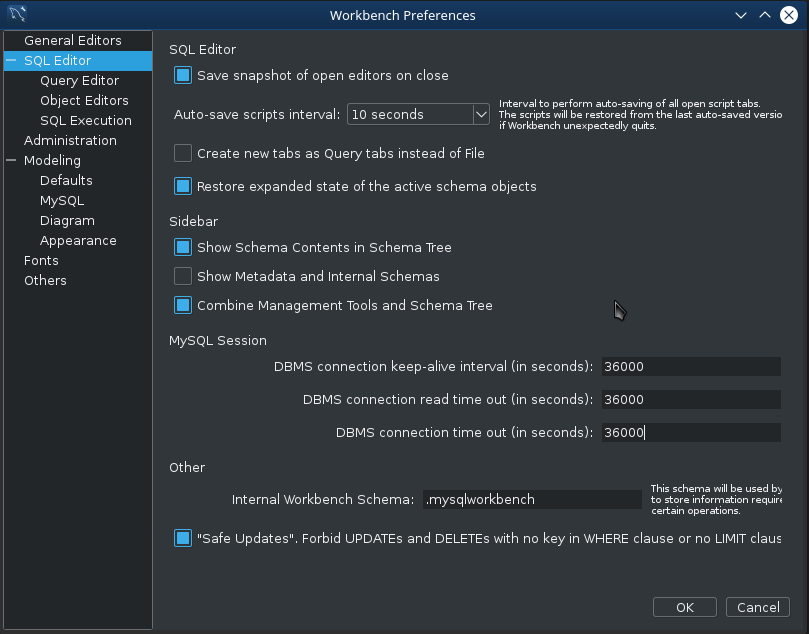
\includegraphics[width=0.6\textwidth]{mysql_wb_settings}
	\caption{MySQL Workbench: Setting timeout values to avoid connection loss}
	\label{fig:mysql_wb_settings}
\end{figure}
% space

\noindent
The next problem was the lack of disk space. 
MySQL by default stores all databases and belonging tables in /var/lib/mysql/, and it also creates temporary backup files 
(where the file size is equal to the size of the current database). 
Since the default folder for temporary files was on /root, the disk space was used up in less than 30 minutes. 
Therefore, two things needed to be done. First, disable the storage of temporary files, and secondly change the storage location for the database. 
The problem when tinkering with the configuration file is that things easily break. 
Which is what happened, and a clean install was needed for both MariaDB and MySQL (the changed settings can be seen in Listing  \ref{lst:mariadb_config_file}). 
The final step was to create symbolic links that linked the database to the  location where the tables were stored 
(this has to be done before creating the tables, if not MySQL  Workbench will store the tables in /var/lib/mysql/)\footnote{
	It should be noted that after an upgrade of MariaDB, MySQL and MariaDB could no longer find the tables, even if they still were in the /home/mysql/ folder. 
	It is therefore advisable to dump the database after inserting all the tables, since it goes a lot faster to restore the database from dump rather than insertion from XML files.
	}. 
% listing of changes made to config file (MariaDB)
\begin{lstlisting}[caption={Changes made to config file: /etc/mysql/my.cnf}, label={lst:mariadb_config_file}] 
# disable storage of temporary files
#tmpdir = /tmp/		  
# disable storage of log files
#log-bin = mysql-bin  

# set directory for storing database files
datadir = /home/mysql 
\end{lstlisting}

% Listing showing the SQL for loading XML row data into MySQL
\begin{lstlisting}[caption={Load XML file into a table in the MySQL database}, label={lst:load_xml_file}, language={SQL}] 
LOAD XML LOCAL INFILE 
path_to_xml_file
INTO TABLE db_table
ROWS IDENTIFIED BY '<row>';
\end{lstlisting}

\noindent
Listing \ref{lst:load_xml_file} shows how the files were loaded into the tables, and the complete database can be seen in Appendix \ref{app:mysql_database}, p.~\pageref{app:mysql_database}. 
Since the Posts table is large (\textasciitilde 29,5 million rows) and it contains both questions and answers, two new tables were created; 
"posvote\_Posts"\footnote{
	The Posts table has a file size of \textasciitilde 43,6 GB, 
	whereas posvote\_Posts file size is \textasciitilde 11,2 GB. 
	negvote\_Posts has a file size of \textasciitilde 1,33 GB.
	} 
and "negvote\_Posts". 
posvote\_Posts contains questions with a score higher then zero (score > 0) and negvote\_Posts contains all questions with a score lower then zero (score < 0).

\section{Development process} 
\label{sec:development_process}
When starting the development, the focus was on retrieving the data from the database, and processing it for text analysis. 
To be able to store all the retrieved columns and the belonging rows without creating object classes, the pandas.DataFrame\footnote{
	Pandas: \url{http://pandas.pydata.org/}.
	} 
was used. 
% add something a bit more detailed about pandas; what makes it good, etc.

The questions retrieved needed to be processed before any analysis could be done. 
The reason for this is because the questions was written as HTML (including HTML entities). 
An example is shown in Listing \ref{lst:unprocessed_question}. 
Every question starts with the <p> tag, and if the question contains code samples, these are wrapped with a <code> tag. 
To convert the HTML text into readable text, a HTML parser class was created (based on answer by \cite{Eloff2009}).
\newpage\noindent
% listing with question before HTML is removed
\begin{lstlisting}[caption={Question before HTML is removed (Question ID: 941156)}, 
label={lst:unprocessed_question}, basicstyle=\small] 
<p>
Why do we need callbacks in ASP.NET or any server side technology?
</p>&#xA;&#xA;<p>One answer can be, to achieve asynchronous calls. 
</p>&#xA;&#xA;<p>But I am not satisfied with this answer.</p>
&#xA;&#xA;<p>Please explain it in a different way.
</p>
&#xA;
\end{lstlisting}
% space

\noindent
To process the questions, CountVectorizer from scikit-learn was used. 
CountVectorizer uses the vocabulary found in the text and counts the frequency of each word \cite{Scikitlearn.org2016b} \cite[see~4.2.3]{Scikitlearn.org2016}. 
When looking at this vocabulary, a lot of of un-important words was found (a lot which came from the code samples) in some of the questions. 
At first all code samples were removed from the text, but later on they were replaced with the value 'has\_codeblock', indicating that this question contained one or more code samples. 
This was achieved by using a combination of lxml\footnote{lxml: \url{http://lxml.de/}} and bs4\footnote{BeatifulSoup: \url{https://www.crummy.com/software/BeautifulSoup/}} (BeatifulSoup). 
lxml was used to construct an XML tree containing all the tags (to be able to retrieve the content by searching for a given tag), and bs4 was used for beautifying the HTML 
(since in some cases an error was thrown complaining about "Missing end tag").
\vspace{0.5em}\newline
However, for some questions, part of the text was lost, and for others, some <code> tags was not removed. 
On inspection, it was found that the trailing text following the <code> samples was stored in a .tail attribute. 
Since the <code> was removed, the .tail attribute was also removed. 
This was fixed by storing the the content of the <code> .tail attribute into its <parent>\footnote{
	It was also necessary to check if the <parent> had a .tail, if not, the .tail attribute had to be set for the <parent> to avoid the error: 
	"NoneType + str: TypeError".
	} 
(where <parent> is the tag that contained the given <code></code>) .tail attribute. 
As for the non-complete removal of <code> tags, this error mostly occurred for code samples that contained XML or HTML code\footnote{
	One example is this question: \\
	\url{http://stackoverflow.com/questions/19535331/print-page-specific-area-or-element}.
	}, 
because the lxml parser failed. 
The solution was to replace the lxml parser with bs4 and just change the content of the <code> tag to the value 'has\_codeblock'.
\vspace{0.5em}\newline
Considering the size of the dataset, and that the source code was hosted on GitHub, I was hesitant to store the training data in a separate file. 
However, when loading 20,000 samples from the database with a 'WHERE' parameter, things tend to go more slow. 
At this point, it was decided to try to dump the loaded data from the database to a file. 
This was achieved by using pandas.DataFrame.to\_csv\footnote{
	pandas.DataFrame.to\_csv: \\
	\url{http://pandas.pydata.org/pandas-docs/stable/generated/pandas.DataFrame.to_csv.html}.
	}. 
At a later point, the unprocessed dataset was also dumped to a CSV file for replicability.
\vspace{0.5em}\newline
Further examination showed that the vocabulary contained a lot of numerical and hexadecimal values, but also a lot of non-English words. 
The numerical and hexadecimal values were replaced using regular expressions to 'has\_hexadecimal' and 'has\_numeric'. 
The non-English words were a bit more troublesome to handle, since these were mainly used to prove a point or show an example of the issue they were having\footnote{ 
	\url{http://stackoverflow.com/questions/856307/wordwrap-a-very-long-string}.
	}. 
Attempts were made to filter them out by using corpus.words.words() and corpus.wordnet.synset() 
from \gls{nltk}\footnote{\url{http://www.nltk.org/}}, and PyEnchant\footnote{\url{http://pythonhosted.org/pyenchant/}}. 
However, WordNet does not have a complete database of all English words, and they all claimed some words were not English even though they were.
The solution turned out to be a lot simpler. 
Instead of creating filters, the CountVectorizer already had one built in. 
By adjusting the minimum document frequency (min\_df) and setting it to 0.01, words that appeared in less 1\% of all documents were ignored.
\vspace{0.5em}\newline
To be able to run the system without relying on an \gls{ide}, making it run from the Terminal using basic command setup seemed like a good idea. 
At first optparse was used, which ironically turned out to be deprecated and replaced by argparse. 
However, the problem was that you could only run one command at a time, whereas I wanted the program to be able to run until exited.
The reason for this was because it needs to load a model before it can make a prediction, in addition the user might want to predict multiple questions. 
This was therefore replaced with a basic while loop that runs until the users enters the exit command. 
The setup used for argparse was kept, so users from *nix system might be more familiar with similar commands (shown in Listing \ref{lst:system_menu}).
At the end, there were some commands that were not added to the menu, since these were mostly used for testing. 
% listing with the available menu commands
\begin{lstlisting}[caption={System menu}, 
label={lst:system_menu}, basicstyle=\small] 
Menu: 
d: Loads default model (if exists) from ./pickle_models
e: Exit the program
h: Displays this help menu
l: Load user created model. Arguments: 
	path: Path to directory with model(s) (e.g. /home/user/my_models/) 
	filename: The models filename 
	suffix: File type - Optional (default: '.pkl')
p: Predict the quality of the entered question. Arguments: 
	question: Question to predict quality of 
t: Train a new model based on an existing (or new) data set. Arguments: 
	path: Path to directory with training data (e.g. /home/user/my_data/) 
	filename: Filename for data set (model name will be the same as this) 
	db_load: Load from database (Enter 0: No, 1: Yes) 
	limit: Limit for database row retrieval (integer) - Optional unless 'db_load' is '1'
u: Create an unprocessed data set based on database content (from database set in dbconfig.py). 
Arguments: 
	filename: Filename for data set (model name will be the same as this) 
	limit: Limit for database row retrieval (integer) 
	feature_detectors: Create singular feature detectors based on data set? (Enter 0: No, 1: Yes) 
	create_model: Create classifier model(s) based on data set? 
	0: No, 1: Unprocessed model, 2: Feature detector model(s) 3: Both (1 and 2)
\end{lstlisting}

\begin{comment}
	Timeline:
		1. Created retrieval method for bad questions from db
			1.1. Using pandas to store data retrieved from db
		2. Added HTML class to remove tags
			Answer source: \url{http://stackoverflow.com/a/925630}
			Source: \url{http://stackoverflow.com/questions/753052/strip-html-from-strings-in-python}
			Accepted answer: "answered May 29 '09 at 11:47 Eloff"
			And comment to this answer by 'pihentagyu aka James Doepp' (May 21 '15 at 17:49)
		3. Tutorial by: \url{http://radimrehurek.com/data_science_python/}
		4. Removal of codeblocks from the question
			4.1 Using BeatifulSoup to processes tags without end-tags			
			4.2 Issues with losing the tail (text after codeblock); attaching it to parent
			4.3 Issue "NoneType + str: TypeError". Caused by parent not having tail. 
				Fixed by adding a .tail and setting it to '' on the <parent>.
			4.4 HTML w/ XML causing issues; parser fails (because parser was also xml, adding xml 
				to beginning of text). Example: 
				\url{http://stackoverflow.com/questions/19535331/print-page-specific-area-or-element}
			4.5 Filtering out questions that failed by adding their index to a temp list, and then 
				removing them from dataset
		5. Issue: Scikit-learn documentation is for v17.1, whereas I was using developer version v18.0
		   (part of the issue was that it wasn't installable, so it was installed from GitHub repo instead)
		   considered switching to libsvm (which wasn't installable through pypi in the beginning)
		6. Instead of removing codeblocks, the text 'has\_codeblock' was added to indicate code was used
			6.1 Stored the processed questions to .csv
		7. Discovered data missing in some questions by looking at the CSV. 
		   Some <code> snippetes weren't removed. Content found after EOF
		   Issue 4.4 was fixed by removing all lxml conversion and using bs4 instead
		8. Questions start with <p>, this was removed by setting all text to be on one line
		9. Removal of numeric and hexadecimal values from text. Issue with trash data, e.g:
			\url{http://stackoverflow.com/questions/856307/wordwrap-a-very-long-string}
		10. Trash data: Using NLTK, NLTK.WordNet and enchant
			10.1 Tested out WordNet, could not discover english words. Does not contain all english words
			10.2 Tested out enchant, but could not in all cases either discover all english words
			10.3 Using Porter stemming to reduce features
			10.? \url{http://www.irfanelahi.com/data-science-document-classification-python/#Lexical-
			Analysis-of-the-Text-Data}
			10.? Setting min\_df=0.01 (ignore those occuring in less then 1\%) - helped a lot 
		11. Stemming of data, model creation and gridsearch with SGD			
		12. Model based on 20,000 samples (10k good, 10k bad) - took approx ~3hours for both models
			Model 1 was for all data (no test set). Model 2 was based on train\_test\_split
		13. Added tags column to the used dataset. Added the unprocessed dataset (but html is removed)
		14. Tested out different SVM algorithms (SVC, SGD and LinearSVC)
			Issue was that I managed to overwrite the .csv, so I had to do everything over again
			took approximately 24-36 hours to complete (+ 3days before hand to make everything run smoothly).
		15. Attempted to use optparse, argparse to make it executable. 
			Problem is that it exits after command is run. Need it to continue running to be able to:
				a) create new (or load existing) model
				b) use model from a) to predict quality of entered question (rinse/repeat)
		16. Used while loop instead (loop until exit entered). shortcuts are the same as with argparse, but 
			without the '-' in front (e.g. instead of -e, just press 'e' to exit)
			
		Additional Notes (which might be relevant for the next section):
		
			- issues with setting up environment, installations, etc
			- switching from "good"/"bad" to +/-1 for class label (bcz libsvm)
			- switching from -10/+50 to -5/+50 to get more separation (and more results for bad)
			
		Potentially useful links:
		
		http://billchambers.me/tutorials/2015/01/14/python-nlp-cheatsheet-nltk-scikit-learn.html
		http://stackoverflow.com/questions/28064634/random-state-pseudo-random-numberin-scikit-learn
		http://stackoverflow.com/questions/35382657/my-pipeline-configuration-for-text-classification-using-
		sklearn-in-python
\end{comment}

\section{Feature sets, attributes and processing}
\label{sec:feature_sets}
When retrieving the questions from the database, the vote score was set to less than -10 for bad question and greater than 50 for good questions (retrieval limit set to 10,000; 20,000 total). 
However, the vote score was set too low for the bad questions, since only 683 rows was returned. 
Therefore, the score was then set to less than -5. 
What was also found when using pandas.Categorical to get an overview (code snippet in Listing \ref{lst:pandas_categorical} and result in Table \ref{tab:pandas_categorical}), 
one can see that for the 10,000 bad questions, the average vote score was -7. This could be an indicator that when a question has a vote score below -5, they are ignored.

\newpage
\begin{lstlisting}[caption={Getting Categorical data from pandas.DataFrame}, 
label={lst:pandas_categorical}, language={Python}, basicstyle=\small] 
from pandas import DataFrame, Categorical

# get statistics from pandas.DataFrame
temp_df = __so_dataframe.loc[:, ("Score", "Body", "Title", 
	"AnswerCount", "length")]
temp_df.loc[:, CLASS_LABEL_KEY] = Categorical(__so_dataframe.loc[:, 
							"label"])

# prints out the questions AnswerCount, Score and length
print(temp_df.groupby("label").describe())
# prints all selected columns
print(temp_df.groupby("label").describe(include='all'))
\end{lstlisting}

\begin{table}[tbp]
	\centering
	\begin{tabular}{| c | c | c | c |c |}
		\hline
		Class 		& Statistics	& AnswerCount		& Score 		& Question length 	\\ \hline
		~ 			& ~ 			& ~  				& ~ 			& ~					\\ \hline
		% Bad Questions
		-1 			& mean 		& 2.0483 			& -7.0275 		& 319.226 		\\ \hline
		~ 			& std 		& 1.3129 			& 2.676 		& 382.115  		\\ \hline
		~ 			& min 		& 0.0 				& -147.0 		& 13.0  		\\ \hline
		~ 			& 25\% 		& 1.0 				& -7.0 			& 153.0 		\\ \hline
		~ 			& 50\% 		& 2.0 				& -6.0 			& 239.0  		\\ \hline
		~ 			& 75\% 		& 3.0 				& -6.0 			& 379.0  		\\ \hline
		~ 			& max 		& 20.0 				& -6.0 			& 13673.0  		\\ \hline
		% space
		~ 			& ~ 		& ~  				& ~ 			& ~				\\ \hline
		% Good Questions
		1 			& mean 		& 11.9379 			& 182.5483 		& 459.329		\\ \hline
		~ 			& std 		& 13.707824			& 317.47217 	& 531.187559  		\\ \hline
		~ 			& min 		& 0.0 				& 51.0 			& 13.0  		\\ \hline
		~ 			& 25\% 		& 6.0 				& 67.0 			& 189.0 		\\ \hline
		~ 			& 50\% 		& 9.0 				& 96.0 			& 328.0  		\\ \hline
		~ 			& 75\% 		& 14.0 				& 173.0 		& 558.0  		\\ \hline
		~ 			& max 		& 518.0 			& 9432.0 		& 18867.0  		\\ \hline
		
	\end{tabular}
	\caption{Results from pandas.DataFrame and pandas.Categorical. -1 is for bad questions (votes < -5), 
		and 1 are for good questions (votes > 50).}
	\label{tab:pandas_categorical}
\end{table}

\begin{table}[tbp]
	\centering
	\begin{tabular}{| c | c | c | c |}
		\hline
		Step & Text processing  & Vocabulary count & CountVectorizer  \\ \hline
		1 	& None 									& 69766 	& analyzer="word" \\ \hline
		2 	& Stop words 							& 69462 	& 
			\shortstack{analyzer="word", \\ stop\_words="english"} \\ \hline
		3 	& \shortstack{Removal of code, 
			hexadecimal \\ and numerical values} 	& 27624 	& 
			\shortstack{analyzer="word", \\ stop\_words="english"} \\ \hline
		4 	& Minimum document frequency 			& 440 		& 
				\shortstack{analyzer="word", min\_df=0.01, \\ stop\_words="english"} \\ \hline
	\end{tabular}
	\caption{Feature reduction steps before and after text was processed.}
	\label{tab:feature_reduction}
\end{table}

To be able to develop some theories on what the difference between good and bad questions was, a total of 200 questions were reviewed (by sorting questions based on 
 votes\footnote{\url{http://stackoverflow.com/questions?sort=votes}}). 
It was easier to see certain patterns in down-voted questions rather than those that were up-voted. 
A repetitive pattern was that many had either no code example, or poorly written code. 
These questions could also show indications of not having tried anything, or that they were based on either homework or school assignments. 
This in turn lead to a hypothesis that if a question contains indicator of word synonyms for homework\footnote{\url{http://www.thesaurus.com/browse/homework}}, 
it would be considered a bad question. 
In addition, some code examples had syntax errors, which made the minimum working example (MWE) not executable. 
Some questions also contained links, either to external resources or indicators of potential duplicates. 
Therefore links was also considered a potentially useful feature. 
Tags was also considered as a feature, which was divided into two: Attached and External tag. 
Attached tags are tags which the user has linked to the question, whereas external tags are all the tags available on \gls{so}.
Version numbering was also considered, but this was not included due to the complexity of writing a proper filtering method to account for all possible variations.
\vspace{0.5em}\newline
Features were added in the same manner as was done for code samples, numerical and hexadecimal values. 
However, there were some issues when attempting to replace the tags and the synonyms for homework.
At first, WordNet was used for synonyms (using wordnet.synset()). 
The only problem was that for the word 'homework', wordnet.synset() only returns ['homework', 'prep', 'preparation'].
Whereas Thesaurus\footnote{\url{http://www.thesaurus.com/browse/homework}} had a lot more suggestions, and was therefore used instead.
Words were selected based on whether or not it was plausible that they could be used in programming related question setting.
A new problem now arose, namely the issue that the word "assignment" did not necessarily need to occur in a homework setting, since it could also be used as a programming word
(e.g. assignment operator\footnote{\url{http://stackoverflow.com/questions/5368258/the-copy-constructor-and-assignment-operator}}).
Therefore features for homework were split into two types: 'has\_homework' and 'has\_assignment'.
\vspace{0.5em}\newline
Tags were without a doubt one of the most annoying features to detect and replace. 
Site tags (or external) are single text values in the database, whereas the question can have up to five tags attached. 
Those attached tags are then separated in the following format: "<c><multi-threading>", which had to be processed by removing the '<' and the '>'.
After the removal, each tag value was added to a list, so that all attached tags was indexed based on the question they belonged to. 
Furthermore, a combination of string replacement and regular expression was needed. 
The regular expression was used for single character tags (e.g. 'C'), and word replacement for longer words.
The reason for this was that when using string replacement, single character tags replaced occurrences even if they appeared in the middle of a word.
If the tags contained characters that could be interpreted as a regular expression (e.g. C++), it would give error about multiple repetitions.
In addition, the tags needed to be sorted based on their length, since for questions that contained tags which included both <C> and <C++>, 
if <C> came first, it replaced the <C++> with 'has\_*\_tag'++. The text also had to be converted to lower-case to ensure proper tag matching. 

\begin{lstlisting}[caption={Replacing tags in the question}, 
label={lst:pandas_categorical}, language={Python}, basicstyle=\small] 
for word in word_set:
	if len(word) == 1:
		# if its only one character (e.g. 'C'), ensure that it is a singular word by using regex
		text = re.sub(r"\b%s\b" % word, replacement_text, text, flags=re.IGNORECASE)
	else:
		text = text.replace(word, replacement_text)
\end{lstlisting}

\section{Selecting estimator and parameters for classification}
\label{sec:estimator_parameter_selection}
Two different classifiers were used, \gls{svc} and \gls{sgd}.
The parameter values that were used for these two are shown in Listing \ref{lst:param_svc} and  \ref{lst:param_sgd}.
These are the default values used in Scikit-learns tutorials \cite{Scikitlearn.org2016k, Scikitlearn.org2016l} (\cite{Huang2008, Maas2011, Zhang2003} used default values for training their system).
\gls{svc} was chosen because this is what I started with in the beginning, based on the tutorial written by \cite{Rehurek2014}.
\gls{sgd} was used in some of Scikit-learns tutorials, and are mostly used for sample sizes greater than 100,000 (see Scikit-learns "roadmap" in Appendix \ref{app:ml_map}, Figure \ref{fig:ml_map}  
 p.~\pageref{app:ml_map}).
Since the sample size in this thesis was only 20,000, the expectation was that \gls{svc} would present better predictions..
% Listing for the SVC parameters
\begin{lstlisting}[caption={Parameters for SVC}, label={lst:param_svc}, language={Python}] 
param_svm = [
{'clf__C': [1, 10, 100, 1000], 'clf__kernel': ['linear']},
{'clf__C': [1, 10, 100, 1000], 'clf__gamma': [0.001, 0.0001], 'clf__kernel': ['rbf']},
{'clf__C': [1, 10, 100, 1000], 'clf__gamma': [0.001, 0.0001], 'clf__kernel': ['sigmoid']},
]
\end{lstlisting}
\clearpage
% Listing for the SGD parameters
\begin{lstlisting}[caption={Parameters for SGD}, label={lst:param_sgd}, language={Python}] 
grid_parameters = {
'vect__min_df': (0.01, 0.025, 0.05, 0.075, 0.1),
'vect__max_df': (0.25, 0.5, 0.75, 0.95, 1.0),
'tfidf__use_idf': (True, False),
'tfidf__norm': ('l1', 'l2'),
'clf__alpha': (0.00001, 0.000001),
'clf__penalty': ('l1', 'l2', 'elasticnet'),
'clf__n_iter': (10, 50, 75, 100),
# 'clf__loss': ('hinge', 'log', 'modified_huber', 'squared_hinge', 'perceptron'),
}
\end{lstlisting}
% editor space
Instead of simply selecting random values for the classifier, exhaustive grid search was selected. 
The downside with using grid search is that it takes a lot of time to train, since all parameters are matched against each other to find the best combination \cite{Bishop2006, Markham2015a}.
An example is presented in Equation \ref{eq:fit_sgd} and \ref{eq:fit_sgd}, showing how many fits the exhaustive search must do before it is completed.
% Equation for the amount of fits for SVC
\begin{equation}\label{eq:fit_svc}
\begin{split}
\text{count(C)} + (\text{count(C)} \cdot \text{count(gamma)}) + (\text{count(C)} \cdot \text{count(gamma)}) \\
\Longrightarrow  \text{result} \cdot \text{cross-validation} = \text{fit\_amount} \\
\Longrightarrow  4 + (4 \cdot 2) + (4 \cdot 2) = 20 \cdot 5 = 100 
\end{split}
\end{equation}
% Equation for the amount of fits for SGD
\begin{equation}\label{eq:fit_sgd}
 5 \cdot 5 \cdot 2 \cdot 2 \cdot 2 \cdot 3 \cdot 4 = 2400 \cdot 5 = 12,000
\end{equation}
% editor space
From Scikit-learn, there are two options for exhaustive search: GridSearchCV and RandomizedSearchCV.
The main difference is that GridSearchCV matches all parameters, and RandomizedSearchCV only uses a selection of the parameters. 
RandomizedSearchCV is faster than GridSearchCV, but as stated in \cite{Markham2015a}, it may give lower scores.
\textcite{Markham2015a} also suggests to start GridSearchCV and then compare the results against RandomizedSearchCV.
Since I wanted to find the best parameters from the selection, GridSearchCV was used. 
However, if the goal was to fine-tune the parameters, RandomizedSearchCV could be more fitting. 
E.g. start with a high spread of values, and after each completed training, select a new set of values based on the best results. 
If the score was then too low, or if you wanted better results, you could use GridSearchCV to find the best parameters.
\vspace{0.5em}\newline
Before running the grid search, the questions were split into two parts, a training set and a test set by using 
 train\_test\_split\footnote{\url{http://scikit-learn.org/stable/modules/generated/sklearn.cross_validation.train_test_split.html}}.
train\_test\_split splits the data randomly, but if the random\_state has a fixed value, data will be split the same way (replicability).
For the grid search, cross validation was also included, using StratifiedKFold with 5-folds.
StratifiedKFold was selected because it is often used for classification tasks \cite{Kononenko2007}.
Cross-validation splits data into k-folds, where training is done on k-1 folds, and then evaluated against the last fold \cite{Bishop2006}.
This means that only 80\% of the 16,000 questions is used for training (12,800 questions for training, and 3,200 for evaluation).
After the training was completed, the classifier models prediction accuracy was evaluated by using the test set.
%\vspace{0.5em}\newline
 
	
	\chapter{chapter4}
	%\chapter{Discussions}
\label{chap:chapter5}

\todo[inline]{Working on re-writing \ref{sec:feature_classifier_results} and re-writing \ref{sec:limitations_and_issues}}

\section{Data set and Question selection}
\label{sec:data_and_testing}
The dataset was retrieved from Stack Exchange Archive \cite{StackExchange2016}, and contains all the data posted since the beginning in 2008. 
In this thesis, only the data for \gls{so} was used, specifically the posted questions.
A simplified overview is shown in Table \ref{tab:dataset_overview_so}, listing questions based on vote score. 

\begin{table}[!h]%[tbp]
	\centering
	\begin{tabular}{| c | c | c | c | c | c |}
		\hline
		~				& Amount		& Oldest		& Newest		& Vote (lowest)		& Vote (highest)	\\ \hline
		Votes < 0		& 659,955		& 06.08.2008	& 06.03.2016	& -147				& -1				\\ \hline
		Votes = 0		& 5,256,105		& 06.08.2008	& 06.03.2016	& 0					& 0					\\ \hline
		Votes > 0		& 5,286,971		& 31.07.2008	& 06.03.2016	& 1					& 13845				\\ \hline
		All questions	& 11,203,031	& 31.07.2008	& 06.03.2016	& -147				& 13845				\\ \hline
	\end{tabular}
	\caption{Overview of the questions in the Stack Overflow dataset.}
	\label{tab:dataset_overview_so}
\end{table}
As previously mentioned in Section \ref{sec:feature_sets}, the value used to extract the questions was set to -5 and +50. 
The problem with these values are that they were simply selected. 
Originally, the value for bad questions was -10, which were then changed to -5, because -10 only retrieved 683 rows (and I wanted 10,000 samples for both question types).
However, as can be seen from Table \ref{tab:dataset_overview_so}, +50 is most likely a too low value for the good questions. 
To get more representative results, three different alternatives could be considered.
\vspace{0.5em}\newline
The first alternative is the easiest. 
If you are only interested in a set sample size, then you could simply retrieve the amount sorted by score.
If you want 10,000 of each, you would then get the 10,000 that are scored highest (or lowest).
The second alternative would be to get a set limit based on the actual score, by using the mean or average.
For all the questions of a given type, retrieve the average and then select questions which has a score higher (or lower) than the average.
The third alternative would be to use quartiles. 
Quartiles is measured by a given percentage of the observations, where each quartile represents 25\%; 
Q$_{1}$ (25\%), M (median, 50\%) and Q$_{3}$ (75\%) \cite{Hagen2011}.
The equation to calculate the quartiles are shown in Equation \ref{eq:quartile1} - \ref{eq:quartile3}.
% equation: Quartile 1
\begin{equation}\label{eq:quartile1}
Q_{1} = \frac{(n + 1)}{4}
\end{equation}
% equation: Quartile 2
\begin{equation}\label{eq:quartile2}
M = \frac{(n + 1)}{2}
\end{equation}
% equation: Quartile 3
\begin{equation}\label{eq:quartile3}
Q_{3} = \frac{3 \cdot (n + 1)}{4}
\end{equation}
As previously mentioned in Section \ref{sec:feature_sets}, there was no clear indicator for the good questions. 
Some consisted only of two sentences, e.g. "I committed the wrong files to Git. How can I undo this commit?"\footnote{
	This question currently have a score of 10,406: \\ 
	\url{http://stackoverflow.com/questions/927358/how-do-you-undo-the-last-commit}.
}. Common for many of the top-voted questions is that they are short, but that is not the case for all of them\footnote{
	One example is this question, with a score of 3,009: \\
	\url{http://stackoverflow.com/questions/826782/css-rule-to-disable-text-selection-highlighting}.
}.
There is also what I would call a bias factor. 
If enough people have the same problem, then it will automatically become a good question. 
Not because of the questions quality, but simply because many will encounter it (e.g. Bugs, \gls{ide} behaviour, tweaks, etc).
The same can be said for bad questions. 
In many cases, a question is bad not because of the question that is asked, but simply because it does not follow the guidelines. 
If a question is a duplicate, it is automatically voted for closure, and will in most cases receive multiple down-votes. 
Questions which gives a hint of being school related will also receive down-votes, mainly because \gls{so} targets professionals and experts. 
\gls{so} is neither a fan of unnecessary text like greetings and gratefulness \cite{CommunityWiki2016a,Heyer2012}.
\vspace{0.5em}\newline
Is \gls{so} fit for measuring question quality?
In a closed domain setting, the answer is yes. 
However, as mentioned, what type of quality being measured must be taken into consideration. 
As it is, the system would not be useful for an educational setting, because it bases its prediction on questions asked on \gls{so}.
If a student were to ask the system a question, it might respond saying that this is a bad question (but the result may be based on the fact that it is a duplicate).
For an educational setting, a better solution would be to develop a system similar to the one in \cite{Lezina2013}.
With the current state of the system (if it were to be used), it would be more appropriate to use it as a measurement tool for new \gls{so} questions, rather then general question quality.
\vspace{0.5em}\newline
Considering the amount of data this data set provides, there is a lot of research that could be used in relation to \gls{ai} and \gls{ml} development. 
One example is \textcite{Schutte2016}, who used the same data set to build an auto-complete for Javascript. 
When taking Big Data into consideration, a question has also been presented on whether or not it is the data, and not the algorithm which improves \gls{ai}~\cite{Klein2016,SpaceMachine.net2016,Wissner-Gross2016}.


\section{Feature and classifier results}
\label{sec:feature_classifier_results}
A total of six features were detected and converted from each question. 
These features were code samples\footnote{
	Nothing was done to the content of the code sample, it was only removed and replaced with 'has\_codeblock'.
}, 
hexadecimal, numerical, synonyms for homework and tags. 
As mentioned in Section \ref{sec:feature_sets}, homework and tags contained two feature types. 
One problem with the external tags (all tags listed on the given site), was that it replaced even normal words\footnote{
	For a visualization of how bad it was, see Figure \ref{fig:tag_features_raw} and \ref{fig:tag_features_external} in Appendix \ref{app:various_screenshots}, p.~\pageref{app:various_screenshots}.
	See also the files "\emph{training\_data\_10000\_unprocessed\_UP\_has\_tags.csv}" and "\emph{training\_data\_10000\_unprocessed\_has\_tags.csv}", found in \\ 
	\emph{./IMT4904\_MasterThesis\_Code/extraction\_sets/}.
} (e.g. "this", "can", "let", etc).
Since the external tags and the word "assignment" was conflictive, these were only included when creating classifier models for the singular feature detectors\footnote{
	The singular feature detectors are based on the premise that each feature should be tested individually, and none of the other feature detectors should be used in the model creation process.
}.
\vspace{0.5em}\newline
To be able to compare if a feature would have an impact, the creation of classifier models was divided into three parts. 
In the first part, the raw, unprocessed data set was used to create a classifier model by using GridSearchCV. 
The only modification done to the data was removing the HTML and converting the text to lower-case. 
In the second part, the best parameter values from the unprocessed classifier model was used to create new models for the singular feature detectors.
This ensures that a correct comparison can be made, since the results for both models are based on the same values. 
If they were all trained separately with GridSearchCV, there is a risk that it would select other parameters for the model.
The last part consisted of using all the features, both with the values from the unprocessed classifier model, and using GridSearchCV to select the best parameters.
Porter stemming was also included, but this was only used for the last classifier model.
The confusion matrices for each classifier model is presented in Appendix \ref{app:confusion_matrix}, \pageref{app:confusion_matrix}.
\vspace{0.5em}\newline
The results for the first and second part of the training is shown in Table \ref{tab:singular_feature_detector_so}.
In this table, all classifiers have been trained using the same parameter settings, based on parameters found from the grid search on the unprocessed data set.
Without doing anything to the questions, the accuracy is already at 79.9\%.
The two features that sticks out the most is Numerical and Tags. 
Numericals accuracy score is 80.55\%, which is better than the unprocessed, and Tags accuracy score is almost 4\% lower than the unprocessed.
However, the results for both Homework and Tags are questionable, because they contain features (external and homework) not represented in the classifier for all the features.
Furthermore, the total number of questions containing Homework is only 374 (including the assignment feature), and Hexadecimal is only present in 160 questions 
(see Table \ref{tab:comparison_of_feature_occurences_only} and \ref{tab:amount_of_singular_questions_processed}).
This means that if Hexadecimal was not a feature, it would not even be included (because the min\_df is set to exclude words appearing in less than 1\% of the questions).
Therefore, Hexadecimal is not a good feature which is shown by the accuracy score in Table \ref{tab:singular_feature_detector_so} and \ref{tab:comparison_of_feature_occurences_only} 
(this is also shown in the confusion matrix in the Appendix).
To get a more representative score for Homework and Tags, an additional classifier model should have been made using only the homework features and the attached tags.
Overall, the only feature that had an increase in its prediction accuracy was the classifier for Numerical (only 375 misclassified as bad).
%The numerical feature is the only feature making a difference, with an equal classification prediction for bad, and even better for good (only 375 misclassified as bad).
% table showing the results for all singular feature detectors, for all questions
\begin{table}[!h]%[tbp]
	\centering
	\begin{tabular}{| c | c |}
		\hline
		~ 				& Accuracy Score	\\ \hline
		Code block 		& 79.17\%			\\ \hline
		Hexadecimal		& 79.90\%			\\ \hline
		Homework 		& 79.90\%			\\ \hline
		Links			& 79.35\%			\\ \hline				
		Numerical		& 80.55\%			\\ \hline
		Tags			& 76.17\%			\\ \hline
		All features	& 79.07\%			\\ \hline
		Unprocessed		& 79.90\%			\\ \hline
	\end{tabular}
	\caption{Classifier results based on the parameters found for the raw (unprocessed) questions. Classifier=SVC, with Kernel=RBF, C=1000 and Gamma=($\gamma$) 0.0001}	
	\label{tab:singular_feature_detector_so}
\end{table}
\vspace{0.5em}\newline
It would also be interesting to compare the unprocessed against each feature detector for the questions containing it.
Following the same basis as the previous part, new classifier models were made, but this a new grid search was executed for each feature. 
This way, the classifier would be adjusted to the number of questions for each feature. 
The results from this training is displayed in Table \ref{tab:comparison_of_feature_occurences_only}, and the confusion matrix is presented in Appendix \ref{app:conf_matrix_singular_only}, 
p.~\pageref{app:conf_matrix_singular_only}). 
One thing that needs to be taken into consideration is the total sample size that was used for training and testing. 
When all questions were used, a total of 16,000 questions was used for training and 4,000 used for evaluation, which is not the same used here.
The number of questions that contained each feature is shown in Table \ref{tab:amount_of_singular_questions_processed}, and the number used for training and evaluation (test set) 
is shown in Table \ref{tab:questions_used_for_singular_training}.
\vspace{0.5em}\newline
One thing that is clear is how much effect the external tags has. Tags appear in 19,967 questions, whereas the detector for all features only appears in 17,558.
This means that at least 2,409 contains external tags, and that if they were to be included, a filtering mechanism would be needed (e.g. ignoring everything that could be considered a word).
The feature for code blocks now have a higher accuracy than the unprocessed, and is better at classifying bad questions. 
This could indicate that questions including a lot of code samples is not a good question\footnote{
	There was no analysis done on the code samples, but during the development, I noticed that some questions also used the <code> tag on words like "Integer" and "Double".
}.
Numerical now has a worse accuracy than the unprocessed.
However, there are two things worth mentioning. 
First, the classifier for Numerical is only trained on 9,024 questions, instead of 20,000.
Second, as can be seen in Table \ref{tab:questions_used_for_singular_training}, only 30\% of the training data are good questions. 
When also looking at the confusion matrix (Appendix \ref{app:conf_matrix_singular_only}, p.~\pageref{app:conf_matrix_singular_only}), it predicts more questions as bad.
\begin{table}[!h]%[tbp]
	\centering
	\begin{tabular}{| c | c | c | c | c | c |}
		\hline
		~				& Unprocessed			& Feature						& C				& Gamma ($\gamma$)	& Kernel	\\ \hline
		Code block	 	& Accuracy: 78.84\%		& Accuracy: 79.04\%				& 1				& N/A				& Linear 	\\ \hline
		Hexadecimal		& Accuracy: 81.25\%		& Accuracy: 81.25\%				& 1				& N/A				& Linear	\\ \hline
		Homework 		& Accuracy: 84.00\%		& Accuracy: 82.67\%				& 1				& N/A				& Linear	\\ \hline
		Links			& Accuracy: 83.72\%		& Accuracy: 81.78\%				& 1				& N/A				& Linear	\\ \hline		
		Numerical		& Accuracy: 80.22\%		& Accuracy: 79.66\%				& 1000			& 0.0001			& RBF		\\ \hline
		Tags			& Accuracy: 79.36\%		& Accuracy: 76.46\%				& 1000			& 0.0001			& RBF		\\ \hline
		All features	& Accuracy: 79.24\%		& Accuracy: 79.15\%				& 1000 			& 0.0001			& RBF 		\\ \hline
	\end{tabular}
	\caption{Comparison of raw data set (unprocessed) and singular features, for questions containing the given feature. Classifier: SVC.}
	\label{tab:comparison_of_feature_occurences_only}
\end{table}
% amount of questions used for training and evaluation
\begin{table}[!h]%[tbp]
	\centering
	\begin{tabular}{| c | c | c | c |}
		\hline
		~ 					& Bad: -1			& Good: 1		& Total		\\ \hline
		Code block			& 5,090				& 4,765			& 9,855		\\ \hline
		Hexadecimal			& 109				& 51			& 160		\\ \hline
		Homework			& 261				& 113			& 374		\\ \hline
		Links				& 778				& 1,798			& 2,575		\\ \hline
		Numerical			& 5,804				& 3,220			& 9,024		\\ \hline
		Tags				& 9,987				& 9,980			& 19,967	\\ \hline
		All features		& 8,466				& 9,092			& 17,558	\\ \hline
	\end{tabular}
	\caption{The number of questions containing the given feature.}
	\label{tab:amount_of_singular_questions_processed}
\end{table}
% overview of the amount of questions used to train each feature (using only questions containing the given feature)
\begin{table}[!h]%[tbp]
	\centering
	\begin{tabular}{| c | c | c | c | c | c |}
		\hline
		~ 					& Training: -1		& Training: 1		& Evaluation: -1	& Evaluation: 1	\\ \hline
		Code block			& 4102				& 3782				& 988				& 983			\\ \hline
		Hexadecimal			& 88				& 40				& 21				& 11			\\ \hline
		Homework			& 205				& 94				& 56				& 19			\\ \hline
		Links				& 627				& 1433				& 151				& 365			\\ \hline
		Numerical			& 4650				& 2569				& 1154				& 651			\\ \hline
		Tags				& 8002				& 7971				& 1985				& 2009			\\ \hline
		All features		& 6795				& 7251				& 1671				& 1841			\\ \hline
	\end{tabular}
	\caption{The number of questions used for evaluation. Bad questions: -1, Good questions: 1.}
	\label{tab:questions_used_for_singular_training}
\end{table}
\vspace{0.5em}\newline
Table \ref{tab:unprocessed_vs_all_feature_detectors_svc_so} shows a comparison between the classifier for unprocessed and all features. 
This also includes a comparison of stemmed vs non-stemmed features. 
There were two stemmers that were considered, Porter and Lancaster.
Lancaster is based on Porter, but is more aggressive, and what I experienced was that words which was not even of the same root (e.g. 'user' and 'using' both became 'us') \cite{Textprocessing.com2016}.
The expectation was that stemming would enhance the prediction and increase the prediction accuracy, but this was not the case. 
When compared with the unprocessed, the accuracy score was 3.93\% lower, and 3.15\% lower than the data set with all feature detectors without stemming.
\begin{table}[!h]%[tbp]
	\centering
	\begin{tabular}{| c | c | c | c |}
		\hline
		~ 					& Unprocessed			& All features			& All features (no stemming)	\\ \hline
		Score 				& 79.90\%				& 75.97\%				& 79.15\%						\\ \hline
		Gamma ($\gamma$)	& 1e$^{-04}$ (0.0001)	& 1e$^{-03}$ (0.001)	& 1e$^{-03}$ (0.001) 			\\ \hline
	\end{tabular}
	\caption{Comparison of the classifier for the raw (unprocessed) questions vs. questions with all features. Classifier: SVC, Kernel=RBF and C=1000.}
	\label{tab:unprocessed_vs_all_feature_detectors_svc_so}
\end{table}
\vspace{0.5em}\newline
Table \ref{tab:unprocessed_vs_all_feature_detectors_sgd_so} shows a comparison between unprocessed and all features (stemmed) using the \gls{sgd} classifier.
A full exhaustive search was also ran on the unprocessed, but this is omitted because it resulted in the same values as for loss='log'.
The reason loss was set to 'log' is because you can then get a probability score when using prediction.
Probability was desired, because when a user then enters a new question to predict, the output would also contain the probability and not just "This is a good/bad question".

\todo[inline]{continue re-writing from here}

As expected, when comparing Table \ref{tab:unprocessed_vs_all_feature_detectors_svc_so} with Table \ref{tab:unprocessed_vs_all_feature_detectors_sgd_so}, \gls{svc} did get a slightly higher score.
The difference is barely notable, since the classifier for the unprocessed \gls{svc} achieved a score of 79.90\% vs. \gls{sgd} which achieved 79.87\% (only 0.3\% difference).
Whereas for the classifier using all features, \gls{svc} achieved a score 75.97\% and \gls{sgd} achieved 75.55\% (0.42\% difference). 
This could indicate that if one were to increase the sample size to 30,000 or higher, \gls{sgd} could be a better classifier.


% confusion matrix part
One thing that is interesting is the comparison of the stemmed and non-stemmed classifiers for the \gls{svc}.
The stemmed classifier has the worst prediction, but the non-stemmed classifier using its own parameters have better prediction for bad questions.
The \gls{sgd} is better at predicting bad questions, but performs worse for good.
When comparing the unprocessed \gls{sgd} classifier against the one using all features, it is much better at predicting good questions.


\begin{table}[!h]%[tbp]
	\centering
	\begin{tabular}{| c | c | c |}
		\hline
		~				& Unprocessed (loss='log')	& All features (loss='log')	\\ \hline
		Score 			& 79.87\%					& 75.55\%					\\ \hline
		Min DF 			& 0.01						& 0.01						\\ \hline
		Max DF 			& 0.5						& 0.75						\\ \hline
		Use IDF			& False						& True						\\ \hline
		Alpha 			& 1e$^{-05}$ (0.00001)		& 1e$^{-05}$ (0.00001)		\\ \hline
		Normalization 	& l2						& l2						\\ \hline		
		Penalty 		& elasticnet				& l2						\\ \hline
		Iteration 		& 50						& 100						\\ \hline
		Loss 			& log						& log						\\ \hline		
	\end{tabular}
	\caption{Comparison of the classifier for the raw (unprocessed) questions vs. questions with all features. Classifier: SGD.}
	\label{tab:unprocessed_vs_all_feature_detectors_sgd_so}
\end{table}
%\vspace{0.5em}\newline


\todo[inline]{move or delete this paragraph}
In Appendix \ref{app:confusion_matrix}, \pageref{app:confusion_matrix}, the confusion matrices for all these are listed. 
The confusion matrix is based on the test set that was created using train\_test\_split.
These show a clear indication that the system is much better at predicting bad questions, then good.
This also explains why it was easier to spot the bad questions, rather than a good one when attempting to find features. 
\\

\todo[inline]{this is not intended to be in the final version, just commentary before re-write}
To see if the system was indeed expandable for communities in \gls{se}, Tex.StackExchange was also tested to see which would be more predictive 
(tables are shown in Appendix \ref{app:tables_tex}, p.~\pageref{app:tables_tex}). 
The results clearly shows that \gls{so} is more predictive, given the amount of data available when compared to Tex.StackExchange\footnote{
	However, it should be noted that this dataset was downloaded in August 2015, but the latest post in that database was from 2014.
}




\clearpage
\section[Artificial Intelligence Methods]{\glsentrylong{ai} (\glsentryshort{ai}) Methods}
\label{sec:ai_methods}

\todo[inline]{main goal is to write about alternative methods and potential limitations with using svm, etc.}


\begin{comment}

For Discussion chapter:
--------------------

% Re-write and use what ever fits
In the \gls{bow} model, only single words or word stems are used as features for representing document content. 
The issue is that learning algorithms are restricted to detecting patterns in the used terminology only, while ignoring conceptual patterns. 
List of weaknesses with using \gls{bow} (1-3 addressed issues on a lexical level, and 4 conceptual level):
\begin{enumerate}
\item Multi-Word Expressions with an own meaning like "European Union" are chunked into pieces with possibly very different meanings like "union".
\item Synonymous Words like "tungsten" and "wolfram" are mapped into different features.
\item Polysemous Words are treated as one single feature while they may actually have multiple distinct meanings.
\item Lack of Generalization: there is no way to generalize similar terms like "beef" and "pork" to their common hypernym "meat".
\end{enumerate}
WordNet database organizes simple words and multi-word expressions of different syntactic categories into so called synonym sets (synsets), 
each of which represents an underlying concept and links these through semantic relations. \\
Conceptual Document Representation:
\begin{itemize}
\item Candidate Term Detection: Strategy built on the assumption that if you find the longest multi-word expressions in the text, 
the lexicon will lead to a mapping to the most specific concept for that word (instead of querying single words, which may lead to wrong mapping).
\item Syntactical Patterns:Analysis by using POS-tagging.
\item Morphological Transformations: Entry form, base form reduction. 
Stemming if the first query for the inflected forms on the original lexicon turned out unsuccessful.
\item Word Sense Disambiguation (WSD): A lexical entry for an expression does not necessarily imply a one-to-one mapping to a concept in the ontology. 
\item Disambiguate an expression versus multiple possible concepts.
\item Generalization: Going from specific concepts in the text to general concept representations. Mapping words based on generalization (up to a certain level).
\end{itemize}
\cite{Bloehdorn2004}

% Re-write and use what ever fits
\gls{qc}: predict the entity type of the answer of a natural language question, mostly achieved by using machine learning. 
Used Latent Semantic Analysis (LSA) technique to reduce the large feature space of questions to a much smaller and efficient feature space. 
Two different classifiers: Back-Propagation Neural Networks (BPNN) and Support Vector Machines (SVM). 
Found that using LSA on question classification made it more time efficient and improved classification accuracy by removing redundant features. 
Discovered that when the original feature space is compact and efficient, its reduced space performs better than a large feature space with a rich set of features. 
They also found that in the reduced feature space, BPNN was better than SVM.  
Competitive with state-of-the-art, even though they used smaller feature space.
\cite{Loni2011}

Sentiment and such: \cite{Maas2011}	

------------------------

Note to self: Map graph over feature impact (unprocessed, singular, all)
Also add in estimated training time for exhaustive search (e.g. ~120 minutes for SVC vs ~100 for SGD over 16k questions (since 4k = test)). 


% could be re-phrased into "in this paper, they define question analysis with two different approaches..."
In the paper by \textcite{Toba2011}, they experiment with the use of statistical learning to find the expected answer pattern for factoid \gls{qa} pairs. 
E.g. if you ask someone where a certain event took place, the answer pattern would be a location. 
They group question analysis into two approaches; pattern-based (high precision, low recall) and \gls{ml} (high recall, 
low precision\footnote{
Low precision can occur if the feature sets are not fitted well enough during classifier training 
\cite[p.~283]{Toba2011}.
}). 
Pattern-based would match word sequences against a set of patterns (e.g. regular expressions), whereas \gls{ml} would be based on the accuracy of the classifier 
(e.g. lexical or linguistic feature sets). 
% editor space
The retrieval of \gls{qa} pairs is done by using a statistical relation framework: Bayesian Analogical Reasoning (BAR). 
Features sets are extracted from the training set by use of binary values checking if the question contains a given question word. 
The BAR framework then learns the related features and computes the estimation for them. 
Thereafter \gls{qa} pairs are retrieved from the testing set and compared against the training set. 
Afterwards, the \gls{qa} pairs that have identical question words are identified, and overlapping pairs are grouped according their named entity group.
To retrieve named entities, they used two different recognizers. 
The first was Stanford (extracts the person, organization and location), and the second was dictionary based (extract number entities and fine-grained noun-based entities). 
Question words were extracted by building a question word list from the training set (achieved by using Stanford Part-of-Speech (POS) tagger). 
Then for each question, look for the appearance of the question word to create the feature set.
Mapped named-entities.
\cite{Toba2011}

\end{comment}

\clearpage
\section{Limitations and other issues}
\label{sec:limitations_and_issues}
\todo[inline]{This whole section will be re-written}
One of the major issues was the fact that the latest development version was used instead of the stable one.
The question became at one point whether or not a switch should be made from using the development version into the stable version.
There were two things that needed to be taken into consideration. 
First of all, it was unknown when this development version would become the next stable one.
If the development version became the new stable version, a lot of alterations would have to be made to the source code.
Furthermore, for the long term, if this system would become successful, it would be easier to maintain in the future if it relied on the latest version.
\vspace{0.5em}\newline
When you are only one person with only one computer there is a certain limitation to how much work can be done simultaneously.
A lot of time were spent having to rebuild the database and processing the data (e.g. finding features, replacing it, training classifiers).
To ensure expandability (for the \gls{se} community) and ensuring replicability (having a unprocessed data set), more than once code had to be updated or re-written. 
This easily caused a lot of unforeseen issues.
The worst one was the realization that after the update of the unprocessed data set (changing it to contain HTML like in the database), the HTML was not removed from the text.
The impact was that all the models that were created using the parameters and data from the unprocessed had to be re-trained to get correct results. 
\vspace{0.5em}\newline
One of the more peculiar issues (which I do not have an explanation for), was when the real training started (using the \gls{svc} and GridSearchCV).
The reason that this issue cannot be explained, is because I do not know what caused it to happen.
What happened was that when the training was started, no verbose was printed at all (which was weird considering I had used the same values before and it then gave a verbose output). 
The program ran for hours, without giving any feedback, errors or output. 
\vspace{0.5em}\newline
It took almost three days to find a solution, where part of the solution was switching to Windows (which had its own issues, since x64 is not supported by Numpy).
The main difference was that in Windows, at least verbose was printed, although it only printed verbose once\footnote{
	Verbose was printed once, sometime twice between the first 20 - 60 minutes, then nothing.
	The longest run time that was registered was around 12 hours without any verbose printed.
}.
There were two things that were changed, which finally made it both print verbose and complete the training.
The first part was changing the n\_jobs value to something else than -1. 
By setting n\_jobs=-1, GridSearchCV will run all jobs in parallel, using all logical cores (e.g. on a CPU with 4 physical cores, it will use all 8 logical cores). 
However, multi-threading is not supported in Windows \cite{GS2015}. 
To ensure that progress was made, and that the program had not frozen again, the verbose level was increased.
By increasing the verbose level, you can force the algorithm to print more information about progress, but with an increase in the time it takes to finish \cite{Manuel2015, user29912432014}. 
The most fascinating part was that after increasing the verbose level, it not only printed out continuously, but it even finished training in less than 3 hours!
This have not been tested in Linux, but the reason nothing happened may have been the same which happened for Windows, that it could not utilize all CPU cores\footnote{
	My assumption is that when all the logical cores are used, there is no processing power left for the Operative System (OS). 
	This in turn would then cause an infinite deadlock, since by using all the cores, there is no processing power left for the OS.
	There is also a known issue with parallelization in Linux, see: 
	\url{https://pythonhosted.org/joblib/parallel.html\#bad-interaction-of-multiprocessing-and-third-party-libraries}.
}.






\todo[inline]{either add this to limitation/issues or delete it}


% this could probably be re-used
The most useful resource were of course Scikit-learns tutorials \cite{Scikitlearn.org2016j}\footnote{
	The examples that were worked through can be seen here (as stated in ReadMe, the only thing I have altered is comments and adjustments for v0.18.dev0): \\
	\url{https://github.com/klAndersen/scikit-learn_tutorials}.
} and documentation \cite{Scikitlearn.org2016,Scikitlearn.org2016h}, 
but there were also two other tutorials that proved helpful (\cite{Rehurek2014} and \cite{Elahi2016}).
% this could also probably be re-used
The main problem was that Scikit-learns documentation and most of the tutorials written by others is based on v0.17.1.
Due to various problems with installation in regards to Numpy and Scipy, Scikit-learn had to be installed from GitHub (which is v0.18.dev0).
In the development version, a lot of functions and modules had been re-written and moved, making many tutorials and examples outdated.

 
	
	\chapter{Discussions}
	%\chapter{Discussions}
\label{chap:chapter5}


\begin{comment}

For Discussion chapter:
--------------------

% Re-write and use what ever fits
In the \gls{bow} model, only single words or word stems are used as features for representing document content. 
The issue is that learning algorithms are restricted to detecting patterns in the used terminology only, while ignoring conceptual patterns. 
List of weaknesses with using \gls{bow} (1-3 addressed issues on a lexical level, and 4 conceptual level):
\begin{enumerate}
\item Multi-Word Expressions with an own meaning like "European Union" are chunked into pieces with possibly very different meanings like "union".
\item Synonymous Words like "tungsten" and "wolfram" are mapped into different features.
\item Polysemous Words are treated as one single feature while they may actually have multiple distinct meanings.
\item Lack of Generalization: there is no way to generalize similar terms like "beef" and "pork" to their common hypernym "meat".
\end{enumerate}
WordNet database organizes simple words and multi-word expressions of different syntactic categories into so called synonym sets (synsets), 
each of which represents an underlying concept and links these through semantic relations. \\
Conceptual Document Representation:
\begin{itemize}
\item Candidate Term Detection: Strategy built on the assumption that if you find the longest multi-word expressions in the text, 
the lexicon will lead to a mapping to the most specific concept for that word (instead of querying single words, which may lead to wrong mapping).
\item Syntactical Patterns:Analysis by using POS-tagging.
\item Morphological Transformations: Entry form, base form reduction. 
Stemming if the first query for the inflected forms on the original lexicon turned out unsuccessful.
\item Word Sense Disambiguation (WSD): A lexical entry for an expression does not necessarily imply a one-to-one mapping to a concept in the ontology. 
\item Disambiguate an expression versus multiple possible concepts.
\item Generalization: Going from specific concepts in the text to general concept representations. Mapping words based on generalization (up to a certain level).
\end{itemize}
\cite{Bloehdorn2004}

% Re-write and use what ever fits
\gls{qc}: predict the entity type of the answer of a natural language question, mostly achieved by using machine learning. 
Used Latent Semantic Analysis (LSA) technique to reduce the large feature space of questions to a much smaller and efficient feature space. 
Two different classifiers: Back-Propagation Neural Networks (BPNN) and Support Vector Machines (SVM). 
Found that using LSA on question classification made it more time efficient and improved classification accuracy by removing redundant features. 
Discovered that when the original feature space is compact and efficient, its reduced space performs better than a large feature space with a rich set of features. 
They also found that in the reduced feature space, BPNN was better than SVM.  
Competitive with state-of-the-art, even though they used smaller feature space.
\cite{Loni2011}

Sentiment and such: \cite{Maas2011}	

------------------------

Note to self: Map graph over feature impact (unprocessed, singular, all)
Also add in estimated training time for exhaustive search (e.g. ~120 minutes for SVC vs ~100 for SGD over 16k questions (since 4k = test)). 


% could be re-phrased into "in this paper, they define question analysis with two different approaches..."
In the paper by \textcite{Toba2011}, they experiment with the use of statistical learning to find the expected answer pattern for factoid \gls{qa} pairs. 
E.g. if you ask someone where a certain event took place, the answer pattern would be a location. 
They group question analysis into two approaches; pattern-based (high precision, low recall) and \gls{ml} (high recall, 
low precision\footnote{
Low precision can occur if the feature sets are not fitted well enough during classifier training 
\cite[p.~283]{Toba2011}.
}). 
Pattern-based would match word sequences against a set of patterns (e.g. regular expressions), whereas \gls{ml} would be based on the accuracy of the classifier 
(e.g. lexical or linguistic feature sets). 
% editor space
The retrieval of \gls{qa} pairs is done by using a statistical relation framework: Bayesian Analogical Reasoning (BAR). 
Features sets are extracted from the training set by use of binary values checking if the question contains a given question word. 
The BAR framework then learns the related features and computes the estimation for them. 
Thereafter \gls{qa} pairs are retrieved from the testing set and compared against the training set. 
Afterwards, the \gls{qa} pairs that have identical question words are identified, and overlapping pairs are grouped according their named entity group.
To retrieve named entities, they used two different recognizers. 
The first was Stanford (extracts the person, organization and location), and the second was dictionary based (extract number entities and fine-grained noun-based entities). 
Question words were extracted by building a question word list from the training set (achieved by using Stanford Part-of-Speech (POS) tagger). 
Then for each question, look for the appearance of the question word to create the feature set.
Mapped named-entities.
\cite{Toba2011}

Potentially move "all this failed and went wrong" here
\end{comment}

~\\
To write: \\
Tutorials that I went through \\
Using SGD (based on tutorials from scikit-learn) \\
Testing out different text classification algorithms (SVC, SGD and LinearSVC) \\
Paths, Windows vs. Linux, parallellization, gpu\_count, etc

\section{Data set and Question selection}
\label{sec:data_and_testing}
The dataset was retrieved from Stack Exchange Archive \cite{StackExchange2016}, and contains all the data posted from the beginning. 
In this thesis, only the data for \gls{so} was used, specifically only the posted questions.
A simplified overview is shown in Table \ref{tab:dataset_overview_so}, which lists questions based on score. 

\begin{table}[!h]%[tbp]
	\centering
	\begin{tabular}{| c | c | c | c | c | c |}
		\hline
		~				& Amount		& Oldest		& Newest		& Vote (lowest)		& Vote (highest)	\\ \hline
		Votes < 0		& 659,955		& 06.08.2008	& 06.03.2016	& -147				& -1				\\ \hline
		Votes = 0		& 5,256,105		& 06.08.2008	& 06.03.2016	& 0					& 0					\\ \hline
		Votes > 0		& 5,286,971		& 31.07.2008	& 06.03.2016	& 1					& 13845				\\ \hline
		All questions	& 11,203,031	& 31.07.2008	& 06.03.2016	& -147				& 13845				\\ \hline
	\end{tabular}
	\caption{Overview of the Stack Overflow dataset.}
	\label{tab:dataset_overview_so}
\end{table}
As previously mentioned in Section \ref{sec:feature_sets}, the value used to extract the questions was set to -5 and +50. 
The problem with these values are that they were simply selected. 
Originally, the value for bad questions was -10, which were then changed to -5 because -10 only retrieved 683 rows (and I wanted 10,000 samples for both question types).
However, as can be seen from Table \ref{tab:dataset_overview_so}, +50 is most likely a to low value for the good questions. 
To get better results based on desired quality, there are three options to consider which could improve this.
\vspace{0.5em}\newline
The first is the easiest. If you are only interested in a set sample size, then you could simply retrieve the amount sorted by score.
If you then want 10,000 of each, you would then get the 10,000 that are scored highest (or lowest).
The second option would be to get a set limit based on the actual score, by using the mean or average.
For all the questions of a given type, retrieve the average and then select questions which has a score higher (or lower) than the average.
The third option would be to use quartiles. 
Quartiles is measured by a given percentage of the observations, where each quartile represents 25\%: Q$_{1}$ (25\%), M (median, 50\%) and Q$_{3}$ (75\%) \cite{Hagen2011}.
The equation to calculate the quartiles are shown in Equation \ref{eq:quartile1} - \ref{eq:quartile3}.
% equation: Quartile 1
\begin{equation}\label{eq:quartile1}
Q_{1} = \frac{(n + 1)}{4}
\end{equation}
% equation: Quartile 2
\begin{equation}\label{eq:quartile2}
M = \frac{(n + 1)}{2}
\end{equation}
% equation: Quartile 3
\begin{equation}\label{eq:quartile3}
Q_{3} = \frac{3 \cdot (n + 1)}{4}
\end{equation}
As previously mentioned in Section \ref{sec:feature_sets}, there was no clear indicator for the good questions. 
Some consisted only of two sentences, e.g. "I committed the wrong files to Git. How can I undo this commit?"\footnote{
	This question currently have a score of 10,406: \\ 
	\url{http://stackoverflow.com/questions/927358/how-do-you-undo-the-last-commit}.
}. Common for most of the top-voted are that they are mostly short, however you also have those that are long\footnote{
	One example is this question, with a score of 3,009: \\
	\url{http://stackoverflow.com/questions/826782/css-rule-to-disable-text-selection-highlighting}.
}.
There is also what I would call a bias factor. 
If enough people have the same problem, then it will automatically become a good question. 
Not because of the questions quality, but simply because many will encounter it (e.g. Bugs, \gls{ide} behaviour, tweaks, etc).
The same can be said for bad questions. 
In many cases, a question is bad not because of the question that is asked, but simply because it does not follow the guidelines. 
If a question is a duplicate, it is automatically voted for closure, and will in most cases receive multiple down-votes. 
Questions which gives a hint of being school related will also receive down-votes, mainly because \gls{so} targets professionals and experts. 
\vspace{0.5em}\newline
Is \gls{so} fit for measuring question quality?
In a closed domain setting, the answer is yes. 
However, as mentioned, what type of quality being measured must be taken into consideration. 
As it is, the system would not be useful for an educational setting, because it bases its prediction on questions asked on \gls{so}.
If a student were to ask the system a question, it might respond saying that this is a bad question (but the result may be based on the fact that it is a duplicate).
For an educational setting, a better solution would be to develop a system similar to the one in \cite{Lezina2013}.
With the current state of the system (if it were to be used), it would be more appropriate to use it as a measurement tool for new \gls{so} questions, rather then general question quality.

\section{Development}
\label{sec:development}
There was a lot of back and forth during the development, with a lot of time being invested in properly understanding how to use Scikit-learn.
The most useful resource were of course Scikit-learns tutorials \cite{Scikitlearn.org2016j}\footnote{
	The examples that were worked through can be seen here (as stated in ReadMe, the only thing I have altered is comments and adjustments for v0.18.dev0): \\
	\url{https://github.com/klAndersen/scikit-learn_tutorials}.
	} and documentation \cite{Scikitlearn.org2016,Scikitlearn.org2016h}, 
but there were also two other tutorials that proved helpful (\cite{Rehurek2014} and \cite{Elahi2016}).
The main problem was that Scikit-learns documentation and most of the tutorials written by others is based on v0.17.1.
Due to various problems with installation in regards to Numpy and Scipy, Scikit-learn had to be installed from GitHub (which is v0.18.dev0).
In the development version, a lot of functions and modules had been re-written and moved, making many tutorials and examples outdated.
One example is the code snippet in \cite["In $\lbrack$42$\rbrack$"]{Rehurek2014}, where '\emph{cv=StratifiedKFold(label\_train, n\_folds=5)}' fails, 
because it expects the first argument to be n\_folds\footnote{
	Documentation for v0.17.1: 
	\url{http://scikit-learn.org/stable/modules/generated/sklearn.cross_validation.StratifiedKFold.html}. \\
	Documentation for v0.18.dev0: 
	\url{http://scikit-learn.org/dev/modules/generated/sklearn.model_selection.StratifiedKFold.html}.
}.
\vspace{0.5em}\newline
\textcite{Rehurek2014} used in his example \gls{svc} to train the \gls{svm}, but no explanation to why these parameter values\footnote{
	I later found that these were just the basic numbers used in one of their examples for the grid search: 
	\url{http://scikit-learn.org/stable/auto_examples/model_selection/grid_search_digits.html}.
},
nor how he selected the best parameter from the printout\footnote{
	The score, parameters and estimator can be found by using these attributes: '\emph{best\_score\_}', '\emph{best\_params\_}' and '\emph{best\_estimator\_}'.
} (mine is shown in Listing \ref{lst:svc_tutorial}).

\begin{lstlisting}[caption={Output from SVC tutorial (testing with linear, rbf and sigmoid)}, label={lst:svc_tutorial}] 
[mean: 0.80232, std: 0.01056, params: {'classifier__kernel': 'linear', 'classifier__C': 1}, 
mean: 0.78451, std: 0.01750, params: {'classifier__kernel': 'linear', 'classifier__C': 10}, 
...(15 lines removed)...
mean: 0.71416, std: 0.00101, params: {'classifier__gamma': 0.0001, 'classifier__kernel': 
'sigmoid', 'classifier__C': 1000}]
\end{lstlisting}
Another issue was that since few tutorials had the data sets available, it was hard to compare my results against theirs to (considering version changes).
In Scikit-learns tutorial for text data \cite{Scikitlearn.org2016h}, they have at the end task suggestions, with attached solutions in the Scikit-learn library.
When looking at the solution for the second task (sentiment analysis), I saw that they used \gls{sgd} (see \cite{Scikitlearn.org2016f}).
Looking at the suggested "road map" (see Appendix \ref{app:ml_map}, Figure \ref{fig:ml_map} on p.~\pageref{app:ml_map}), 
I accidentally misread a zero and decided to go with \gls{sgd} instead of \gls{svc}.
\vspace{0.5em}\newline




When understanding more about how GridSearchCV worked and how one could select the best parameters from it, things got back on track. 
However, when comparing it against the \gls{svc}, it turned out that the \gls{svc} got a higher score\footnote{
	A comparison was done on \gls{sgd}, \gls{svc} and LinearSVC using GridSearchCV.
}. 

% something about parameter selection
% something about the results
% something about using probability prediction (e.g. taking twice the time, worse results for SGD, etc.)


\todo[inline]{these tables and listings are temporarily placed here and might be moved into Appendix at a later point.}


\begin{lstlisting}[caption={Parameters for SGD}, label={lst:param_sgd}] 
grid_parameters = {
'vect__min_df': (0.01, 0.025, 0.05, 0.075, 0.1),
'vect__max_df': (0.25, 0.5, 0.75, 0.95, 1.0),
'tfidf__use_idf': (True, False),
'tfidf__norm': ('l1', 'l2'),
'clf__alpha': (0.00001, 0.000001),
'clf__penalty': ('l1', 'l2', 'elasticnet'),
'clf__n_iter': (10, 50, 75, 100),
# 'clf__loss': ('hinge', 'log', 'modified_huber', 'squared_hinge', 'perceptron'),
}
\end{lstlisting}


\begin{lstlisting}[caption={Parameters for SVC}, label={lst:param_svc}] 
param_svm = [
{'clf__C': [1, 10, 100, 1000], 'clf__kernel': ['linear']},
{'clf__C': [1, 10, 100, 1000], 'clf__gamma': [0.001, 0.0001], 'clf__kernel': ['rbf']},
{'clf__C': [1, 10, 100, 1000], 'clf__gamma': [0.001, 0.0001], 'clf__kernel': ['sigmoid']},
]
\end{lstlisting}

\begin{table}[!h]%[tbp]
	\centering
	\begin{tabular}{| c | c | c |}
		\hline
		~ 			& Unprocessed		& Features	\\ \hline
		Score 		& 0.993				& 0.993		\\ \hline
		C			& 1					& 1			\\ \hline
		Kernel		& Linear			& Linear	\\ \hline
	\end{tabular}
	\caption{Comparison of raw data set (unprocessed) and singular feature detectors for Tex.StackExhange (August 2015 data set).}
	\label{tab:singular_feature_detector_tex}
\end{table}


\begin{table}[!h]%[tbp]
	\centering
	\begin{tabular}{| c | c |}
		\hline
		~ 				& Score	\\ \hline
		Code samples 	& 0.783	\\ \hline
		Numerical		& 0.796	\\ \hline
		Hexadecimal		& 0.793	\\ \hline
		Homework 		& 0.794	\\ \hline
		Link			& 0.795	\\ \hline
		Tags			& 0.757	\\ \hline
		Unprocessed		& 0.804 \\ \hline
	\end{tabular}
	\caption{Comparison of raw data set (unprocessed) and singular feature detectors. Using SVC, with Kernel=RBF, C=1000 and Gamma=($\gamma$) 0.001}
	\label{tab:singular_feature_detector_so}
\end{table}


\begin{table}[!h]%[tbp]
	\centering
	\begin{tabular}{| c | c | c | c |}
		\hline
		~ 					& Unprocessed (SVC)	& All features	& All features (no stemming)	\\ \hline
		Score 				& 0.804				& 0.793			& 0.784							\\ \hline
		C					& 1000				& 1000			& 1000							\\ \hline
		Gamma ($\gamma$)	& 0.001				& 0.001			&  0.001							\\ \hline
		Kernel				& RBF				& RBF			& RBF							\\ \hline
	\end{tabular}
	\caption{Comparison of raw data set (unprocessed) and singular feature detectors (SVC)}
	\label{tab:unprocessed_vs_all_feature_detectors_svc_so}
\end{table}

\begin{table}[!h]%[tbp]
	\centering
	\begin{tabular}{| c| c | c | c | c |}
		\hline
		~				& Unprocessed		& Unprocessed (loss='log')		& All features (loss='log')	\\ \hline
		Score 			& 0.8073125				& 0.8071875					& 0.79325					\\ \hline
		Min DF 			& 0.01					& 0.01						& 0.01						\\ \hline
		Max DF 			& 1.0					& 1.0						& 0.75						\\ \hline
		Use IDF			& False					& True						& True						\\ \hline
		Alpha 			& 1e-05					& 1e-05						& 1e-05						\\ \hline
		Normalization 	& l1					& l2						& l2						\\ \hline		
		Penalty 		& l1					& l2						& l2						\\ \hline
		Iteration 		& 100					& 75						& 100						\\ \hline
		Loss 			& hinge					& log						& log						\\ \hline		
	\end{tabular}
	\caption{Comparison of raw data set (unprocessed) and singular feature detectors (SGD)}
	\label{tab:unprocessed_vs_all_feature_detectors_sgd_so}
\end{table}


\begin{table}[!h]%[tbp]
	\centering
	\begin{tabular}{| c | c | c | c | c | c | c |}
		\hline
		~				& Unprocessed		& FEATURE		& C			& Gamma ($\gamma$)	& Kernel	& Amount	 	\\ \hline
		Code samples 	& Score: 0.802		& Score: 0.784	& 1000		& 0.001				& RBF 		& 9,855 		\\ \hline
		Numerical		& Score: 0.834		& Score: 0.815	& 1			& N/A				& Linear	& 9,024			\\ \hline
		Hexadecimal		& Score: 0.859		& Score: 0.883	& 1000		& 0.001				& RBF		& 160 			\\ \hline
		Homework 		& Score: 0.873		& Score: 0.859	& 1000		& 0.001				& RBF		& 374 			\\ \hline
		Link			& Score: 0.885		& Score: 0.838	& 1			& N/A				& Linear	& 2,575			\\ \hline
		Tags			& Score: 0.806		& Score: 0.757	& 1000		& 0.001				& Sigmoid	& 19,967		\\ \hline
		All features	& Score: 0.808		& Score: 0.788	& 1000		& 0.001				& RBF 		& 17,558		\\ \hline
	\end{tabular}
	\caption{Comparison of raw data set (unprocessed) and numerical, for questions that had it.}
	\label{tab:comparison_of_feature_occurences_only}
\end{table}



\section[Artificial Intelligence Methods]{\glsentrylong{ai} (\glsentryshort{ai}) Methods}
\label{sec:ai_methods}
alternative methods and options (e.g. one could have used ann or k-nn, but as shown in\ldots) \\
not sure if this section is relevant?

\section{Implementation Architecture}
\label{sec:implemented_architecture}
discussion on the code that was written and its functionality \\
what worked, what should be updated/changed, etc.

\section{Limitations and other issues}
\label{sec:limitations_and_issues}
why didn't something work as intended? \\
why wasn't X completed/implemented? \\
etc.
 
	
	\chapter{Conclusion/Summary}
	%\chapter{Conclusion/Summary}
\label{chap:chapter6}

\section{Conclusion}
\label{sec:conclusion}
\gls{so} is today a well known \gls{qa} community for programmers, and has existed since late 2008.
\gls{so} can be seen as a gamification system, that awards users for their participation by giving out reputation and badges. 
If the question (or answer) that is posted is considered of good quality by the community, it gets up-voted. 
\gls{so} has a strict policy on what type of questions are allowed to be posted, and it was therefore interesting to see if this could be used to measure question quality. 
\vspace{0.5em}\newline
In this thesis, a data set containing all information posted within the \gls{se} community was acquired.
The data set (downloaded in March 2016) for \gls{so} contains a total of 11,203,031 questions.
Two classifier types were tested, \gls{svc} and \gls{sgd} on a total of 20,000 questions.
The testing was done on both the unprocessed questions and questions containing one or more feature detectors.
The classifier using \gls{svc} had the highest accuracy score, where the Numerical feature got an accuracy score of 80.55\%, but only when trained on all questions. 
The unprocessed got second place, with an accuracy score of 79.90\%.
However, when training the classifiers only on questions that contained the given feature, Numerical got a lower score than the unprocessed.
Which could mean that the feature only did better  for all questions, because it had more questions (and not feature occurrences) to learn from. 
\vspace{0.5em}\newline
The classifier using \gls{sgd} achieved a slightly lower score than \gls{svc}, with an accuracy score of 79.87\%.
This could indicate that the \gls{sgd} would perform better for a larger data set, if the number of questions was increased to 30,000 or more.
The comparison of the confusion matrices for the singular feature detector also show that it is easier to predict bad questions, rather than good.


\section{Further work}
\label{sec:further_work}
Further development of the system would include analysis of the code, to check for syntax errors. 
Sentiment analysis could also be of interest, since \gls{so} does not want greetings or gratefulness in their questions \cite{CommunityWiki2016a}.
For the sentiment analysis, symbol checking would also be included ( e.g. '?', '!', emoticons, etc).
Version numbering is one of the features that were excluded, due to the complexity\footnote{
	A version number can contain numbers, letters and symbols, in addition to including a "v." or "version", or product name.
}.
It would also be interesting to see what results the \gls{sgd} would give when training a classifier on each of the singular features.


\begin{comment}

If these are'nt relevant, just remove them

%\textcite{Stanley2013} - Predicting Tags for StackOverflow Posts

%\textcite{Short2014} - Tag Recommendations in StackOverflow

%\textcite{Wang2013} - An Empirical Study on Developer Interactions in StackOverflow
\end{comment}

 
	
	% bibliography
	\bibliographystyle{ntnuthesis/ntnuthesis}
	\bibliography{../chapters/IMT4904_klAndersen}
	
	%%%%%%%%%%%%%%%%%%%%%%%%%%%%%%%%%%%%%%%%%%%%%%%%%%%%%%%%%%%%%
%% APPENDICES
%%%%%%%%%%%%%%%%%%%%%%%%%%%%%%%%%%%%%%%%%%%%%%%%%%%%%%%%%%%%%
\appendix

\chapter{Appendix}
\label{app:acronyms}
%% acronyms
\printindex
\printglossaries

%\section{Data sets/Statistical Overview}
%\label{app:data_sets}

\clearpage
\section{MySQL Database}
\label{app:mysql_database}
% image of the mysql database
\begin{figure}[ht]
	\centering
    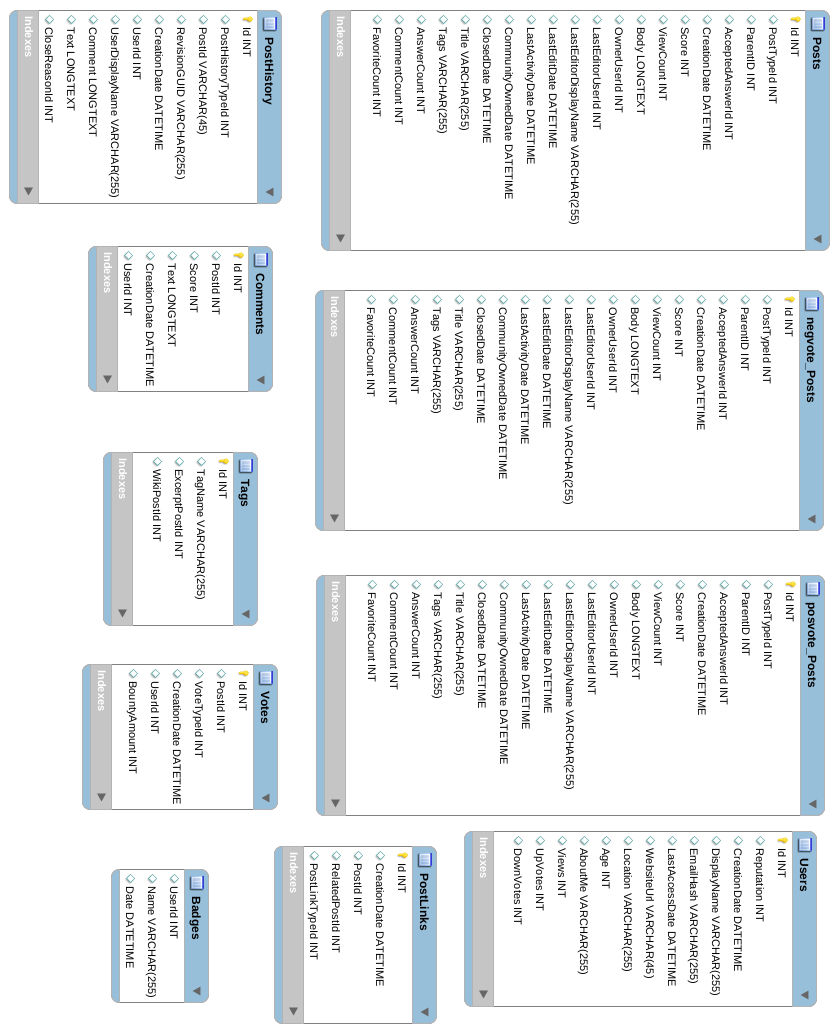
\includegraphics[width=0.8\textwidth]{so_database}
	\caption{MySQL Database used for dataset}
	\label{fig:mysql_database}
\end{figure}

\clearpage
\section{Tex.Stack Exchange: Data set and Features}
\label{app:tables_tex}

%description
\begin{table}[!h]%[tbp]
	\centering
	\begin{tabular}{| c | c | c | c | c | c |}
		\hline
		~				& Amount		& Oldest		& Newest		& Vote (lowest)		& Vote (highest)	\\ \hline
		Votes < 0		& 93			& 22.08.2010	& 10.09.2014	& -14				& -1				\\ \hline
		Votes = 0		& 5,078			& 26.07.2010	& 14.09.2014	& 0					& 0					\\ \hline
		Votes > 0		& 65,919		& 18.08.2008	& 14.09.2014	& 1					& 448				\\ \hline
		All questions	& 71,090 		& 18.08.2008	& 14.09.2014	& -14				& 448				\\ \hline
	\end{tabular}
\caption{Overview of the questions in the Tex.StackExhange (August 2015 data set)}
\label{tab:dataset_overview_tex}
\end{table}

% editor space
\begin{table}[!h]%[tbp]
	\centering
	\begin{tabular}{| c | c | c |}
		\hline
		~ 			& Unprocessed		& Features	\\ \hline
		Score 		& 0.99				& 0.99		\\ \hline
		C			& 1					& 1			\\ \hline
		Kernel		& Linear			& Linear	\\ \hline
	\end{tabular}
\caption{Comparison of raw data set (unprocessed) and feature detectors for Tex.StackExhange (August 2015 data set). Vote score was < 0 for bad and > +7 for good.}
\label{tab:singular_feature_detector_tex}
\end{table}

% description
\begin{table}[!h]%[tbp]
	\centering
	\begin{tabular}{| c | c | c |}
		\hline
		Actual 		& Predicted: -1	& Predicted: 1	\\ \hline
		-1			& 0			& 15				\\ \hline
		1			& 0			& 2004				\\ \hline
	\end{tabular}
	\caption{Confusion Matrix for Tex.StackExhange.}
	\label{tab:confusion_matrix_tex}
\end{table}

% description
\begin{table}[!h]%[tbp]
	\centering
	\begin{tabular}{| c | c | c | c | c |}
		\hline
		~				& Precision		& Recall	& F1-score		& Support	\\ \hline
		-1      		& 0.00			& 0.00		& 0.00			& 15		\\ \hline
		1       		& 0.99			& 1.00		& 1.00			& 2004		\\ \hline
		avg / total		& 0.99			& 0.99		& 0.99			& 2019		\\ \hline
	\end{tabular}
	\caption{Classification report for Tex.StackExhange (August 2015 data set).}
	\label{tab:tex_classification_report}
\end{table}

\clearpage
\section{Confusion Matrices for Stack Overflow}
\label{app:confusion_matrix}
\subsection{Confusion matrices for unprocessed and all feature detectors}

\begin{table}[!htb]
	\caption{Confusion Matrix for unprocessed data set and all feature detectors using the same parameters.}
	\begin{minipage}{.5\linewidth}
		\caption{Unprocessed dataset}
		\centering
		\begin{tabular}{| c | c | c |}
			\hline
			Actual 		& Predicted: -1	& Predicted: 1	\\ \hline
			-1			& 1591			& 403			\\ \hline
			1			& 401			& 1605			\\ \hline
		\end{tabular}
	\end{minipage}%
	\begin{minipage}{.5\linewidth}
		\centering
		\caption{All features}
		\begin{tabular}{| c | c | c |}
			\hline
			Actual 		& Predicted: -1	& Predicted: 1	\\ \hline
			-1			& 1558			& 436			\\ \hline
			1			& 401			& 1605			\\ \hline
		\end{tabular}
	\end{minipage} 
	\begin{minipage}{.5\linewidth}
		\caption{Code blocks}
		\centering
		\begin{tabular}{| c | c | c |}
			\hline
			Actual 		& Predicted: -1	& Predicted: 1	\\ \hline
			-1			& 1547			& 420			\\ \hline
			1			& 413			& 1593			\\ \hline
		\end{tabular}
	\end{minipage}%
	\begin{minipage}{.5\linewidth}
		\centering
		\caption{Hexadecimal}
		\begin{tabular}{| c | c | c |}
			\hline
			Actual 		& Predicted: -1	& Predicted: 1	\\ \hline
			-1			& 1591			& 403			\\ \hline
			1			& 401			& 1605			\\ \hline
		\end{tabular}
	\end{minipage} 
	\begin{minipage}{.5\linewidth}
		\caption{Homework}
		\centering
		\begin{tabular}{| c | c | c |}
			\hline
			Actual 		& Predicted: -1	& Predicted: 1	\\ \hline
			-1			& 1590			& 404			\\ \hline
			1			& 400			& 1606			\\ \hline
		\end{tabular}
	\end{minipage}%
	\begin{minipage}{.5\linewidth}
		\centering
		\caption{Links}
		\begin{tabular}{| c | c | c |}
			\hline
			Actual 		& Predicted: -1	& Predicted: 1	\\ \hline
			-1			& 1548			& 410			\\ \hline
			1			& 416			& 1590			\\ \hline
		\end{tabular}
	\end{minipage} 	
	\begin{minipage}{.5\linewidth}
		\centering
		\caption{Numerical}
		\begin{tabular}{| c | c | c |}
			\hline
			Actual 		& Predicted: -1	& Predicted: 1	\\ \hline
			-1			& 1591			& 403			\\ \hline
			1			& 375			& 1631			\\ \hline
		\end{tabular}
	\end{minipage}%	
	\begin{minipage}{.5\linewidth}
		\caption{Tags}
		\centering
		\begin{tabular}{| c | c | c |}
			\hline
			Actual 		& Predicted: -1	& Predicted: 1	\\ \hline
			-1			& 1508			& 486			\\ \hline
			1			& 467			& 1539			\\ \hline
		\end{tabular}
	\end{minipage}
\end{table}	


\begin{table}[!htb]
	\caption{Confusion Matrix for all features, with and without stemming.}
	\begin{minipage}{.5\linewidth}
		\caption{With stemming}
		\centering
		\begin{tabular}{| c | c | c |}
			\hline
			Actual 		& Predicted: -1	& Predicted: 1	\\ \hline
			-1			& 1558			& 436				\\ \hline
			1			& 525			& 1481				\\ \hline
		\end{tabular}
	\end{minipage}%
	\begin{minipage}{.5\linewidth}
		\centering
		\caption{Without stemming}
		\begin{tabular}{| c | c | c |}
			\hline
			Actual 		& Predicted: -1	& Predicted: 1	\\ \hline
			-1			& 1567			& 427				\\ \hline
			1			& 408			& 1598				\\ \hline
		\end{tabular}
	\end{minipage} 
\end{table}	
\begin{table}[!htb]
	\caption{Confusion Matrix for the SGD classifier, with loss='log'.}
	\begin{minipage}{.5\linewidth}
		\caption{Unprocessed}
		\centering
		\begin{tabular}{| c | c | c |}
			\hline
			Actual 		& Predicted: -1	& Predicted: 1	\\ \hline
			-1			& 1610			& 384			\\ \hline
			1			& 594			& 1412			\\ \hline
		\end{tabular}
	\end{minipage}%
	\begin{minipage}{.5\linewidth}
		\caption{All features with stemming}
		\centering
		\begin{tabular}{| c | c | c |}
			\hline
			Actual 		& Predicted: -1	& Predicted: 1	\\ \hline
			-1			& 1607			& 387			\\ \hline
			1			& 418			& 1588			\\ \hline
		\end{tabular}
	\end{minipage} 
\end{table}	

\begin{comment}
\clearpage
%\subsection{Confusion matrix for singular feature detectors - all questions}

\begin{table}[!htb]
	\caption{Confusion Matrix for singular feature detectors, based on all questions in the data set.}	
	\begin{minipage}{.5\linewidth}
		\caption{Code blocks}
		\centering
		\begin{tabular}{| c | c | c |}
			\hline
			Actual 		& Predicted: -1	& Predicted: 1	\\ \hline
			-1			& 1547			& 420			\\ \hline
			1			& 413			& 1593			\\ \hline
		\end{tabular}
	\end{minipage}%
	\begin{minipage}{.5\linewidth}
		\centering
		\caption{Hexadecimal}
		\begin{tabular}{| c | c | c |}
			\hline
			Actual 		& Predicted: -1	& Predicted: 1	\\ \hline
			-1			& 1591			& 403			\\ \hline
			1			& 401			& 1605			\\ \hline
		\end{tabular}
	\end{minipage} 
	\begin{minipage}{.5\linewidth}
		\caption{Homework}
		\centering
		\begin{tabular}{| c | c | c |}
			\hline
			Actual 		& Predicted: -1	& Predicted: 1	\\ \hline
			-1			& 1590			& 404			\\ \hline
			1			& 400			& 1606			\\ \hline
		\end{tabular}
	\end{minipage}%
	\begin{minipage}{.5\linewidth}
		\centering
		\caption{Links}
		\begin{tabular}{| c | c | c |}
			\hline
			Actual 		& Predicted: -1	& Predicted: 1	\\ \hline
			-1			& 1548			& 410			\\ \hline
			1			& 416			& 1590			\\ \hline
		\end{tabular}
	\end{minipage} 	
	\begin{minipage}{.5\linewidth}
		\centering
		\caption{Numerical}
		\begin{tabular}{| c | c | c |}
			\hline
			Actual 		& Predicted: -1	& Predicted: 1	\\ \hline
			-1			& 1591			& 403			\\ \hline
			1			& 375			& 1631			\\ \hline
		\end{tabular}
	\end{minipage}%	
	\begin{minipage}{.5\linewidth}
		\caption{Tags}
		\centering
		\begin{tabular}{| c | c | c |}
			\hline
			Actual 		& Predicted: -1	& Predicted: 1	\\ \hline
			-1			& 1508			& 486			\\ \hline
			1			& 467			& 1539			\\ \hline
		\end{tabular}
	\end{minipage}
\end{table}	

\end{comment}

\clearpage
\subsection{Confusion matrices for singular feature detectors - occurrence only}
\label{app:conf_matrix_singular_only}

\begin{table}[!htb]
	\caption{Confusion Matrix for singular feature detectors, only for questions containing it.}
	\begin{minipage}{.5\linewidth}
		\caption{Unprocessed}
		\centering
		\begin{tabular}{| c | c | c |}
			\hline
			Actual 		& Predicted: -1	& Predicted: 1	\\ \hline
			-1			& 786			& 202			\\ \hline
			1			& 215			& 768				\\ \hline
		\end{tabular}
	\end{minipage}%
	\begin{minipage}{.5\linewidth}
		\centering
		\caption{Code blocks}
		\begin{tabular}{| c | c | c |}
			\hline
			Actual 		& Predicted: -1	& Predicted: 1	\\ \hline
			-1			& 793			& 195			\\ \hline
			1			& 218			& 765				\\ \hline
		\end{tabular}
	\end{minipage}
	\begin{minipage}{.5\linewidth}
		\caption{Unprocessed}
		\centering
		\begin{tabular}{| c | c | c |}
			\hline
			Actual 		& Predicted: -1	& Predicted: 1	\\ \hline
			-1			& 21			& 0			\\ \hline
			1			& 6				& 5				\\ \hline
		\end{tabular}
	\end{minipage}%
	\begin{minipage}{.5\linewidth}
		\centering
		\caption{Hexadecimal}
		\begin{tabular}{| c | c | c |}
			\hline
			Actual 		& Predicted: -1	& Predicted: 1	\\ \hline
			-1			& 21			& 0				\\ \hline
			1			& 6				& 5				\\ \hline
		\end{tabular}
	\end{minipage} 	
	\begin{minipage}{.5\linewidth}
		\centering
		\caption{Unprocessed}
		\begin{tabular}{| c | c | c |}
			\hline
			Actual 		& Predicted: -1	& Predicted: 1	\\ \hline
			-1			& 52			& 4			\\ \hline
			1			& 8				& 11		\\ \hline
		\end{tabular}
	\end{minipage} 	%
	\begin{minipage}{.5\linewidth}
		\caption{Homework}
		\centering
		\begin{tabular}{| c | c | c |}
			\hline
			Actual 		& Predicted: -1	& Predicted: 1	\\ \hline
			-1			& 50			& 6 			\\ \hline
			1			& 7 			& 12			\\ \hline
		\end{tabular}
	\end{minipage}
	\begin{minipage}{.5\linewidth}
		\caption{Unprocessed}
		\centering
		\begin{tabular}{| c | c | c |}
			\hline
			Actual 		& Predicted: -1	& Predicted: 1	\\ \hline
			-1			& 95			& 56			\\ \hline
			1			& 28			& 337			\\ \hline
		\end{tabular}
	\end{minipage}%
	\begin{minipage}{.5\linewidth}
		\centering
		\caption{Links}
		\begin{tabular}{| c | c | c |}
			\hline
			Actual 		& Predicted: -1	& Predicted: 1	\\ \hline
			-1			& 87			& 64			\\ \hline
			1			& 30			& 335			\\ \hline
		\end{tabular}
	\end{minipage} 
	\begin{minipage}{.5\linewidth}
		\caption{Unprocessed}
		\centering
		\begin{tabular}{| c | c | c |}
			\hline
			Actual 		& Predicted: -1	& Predicted: 1	\\ \hline
			-1			& 1044			& 110			\\ \hline
			1			& 247			& 404			\\ \hline
		\end{tabular}
	\end{minipage}%
	\begin{minipage}{.5\linewidth}
		\centering
		\caption{Numerical}
		\begin{tabular}{| c | c | c |}
			\hline
			Actual 		& Predicted: -1	& Predicted: 1	\\ \hline
			-1			& 1043			& 111			\\ \hline
			1			& 256			& 395			\\ \hline
		\end{tabular}
	\end{minipage} 	
	\begin{minipage}{.5\linewidth}
		\centering
		\caption{Unprocessed}
		\begin{tabular}{| c | c | c |}
			\hline
			Actual 		& Predicted: -1	& Predicted: 1	\\ \hline
			-1			& 1559			& 426			\\ \hline
			1			& 398			& 1611			\\ \hline
		\end{tabular}
	\end{minipage}%
	\begin{minipage}{.5\linewidth}
		\caption{Tags}
		\centering
		\begin{tabular}{| c | c | c |}
			\hline
			Actual 		& Predicted: -1	& Predicted: 1	\\ \hline
			-1			& 1487			& 498			\\ \hline
			1			& 442			& 1567			\\ \hline
		\end{tabular}
	\end{minipage}
	\begin{minipage}{.5\linewidth}
		\caption{Unprocessed}
		\centering
		\begin{tabular}{| c | c | c |}
			\hline
			Actual 		& Predicted: -1	& Predicted: 1	\\ \hline
			-1			& 1284			& 387			\\ \hline
			1			& 342			& 1499			\\ \hline
		\end{tabular}
	\end{minipage}%
	\begin{minipage}{.5\linewidth}
		\caption{All features}
		\centering
		\begin{tabular}{| c | c | c |}
			\hline
			Actual 		& Predicted: -1	& Predicted: 1	\\ \hline
			-1			& 1268			& 403			\\ \hline
			1			& 329			& 1512			\\ \hline
		\end{tabular}
	\end{minipage}
\end{table}	

\begin{comment}
\section{Classification report for Stack Overflow}

\begin{table}[!htb]
	\caption{Classification report for unprocessed data set and all feature detectors using the same parameters.}
	\begin{minipage}{.5\linewidth}
		\caption{Unprocessed dataset}
		\centering
		\begin{tabular}{| c | c | c | c | c |}
			\hline
			~				& Precision		& Recall	& F1-score		& Support	\\ \hline
			-1      		& xxxx			& xxxx		& xxxx			& xxxx		\\ \hline
			1       		& xxxx			& xxxx		& 1x00			& xxxx		\\ \hline
			avg/total		& xxxx			& xxxx		& xxxx			& xxxx		\\ \hline
		\end{tabular}
	\end{minipage}%
	\begin{minipage}{.5\linewidth}
		\centering
		\caption{All features}
		\begin{tabular}{| c | c | c | c | c |}
			\hline
			Precision		& Recall	& F1-score		& Support	\\ \hline
			xxxx			& xxxx		& xxxx			& xxxx		\\ \hline
			xxxx			& xxxx		& 1x00			& xxxx		\\ \hline
			xxxx			& xxxx		& xxxx			& xxxx		\\ \hline
		\end{tabular}
	\end{minipage} 
	\begin{minipage}{.5\linewidth}
		\caption{Code blocks}
		\centering
		\begin{tabular}{| c | c | c | c | c |}
			\hline
			~				& Precision		& Recall	& F1-score		& Support	\\ \hline
			-1      		& xxxx			& xxxx		& xxxx			& xxxx		\\ \hline
			1       		& xxxx			& xxxx		& 1x00			& xxxx		\\ \hline
			avg / total		& xxxx			& xxxx		& xxxx			& xxxx		\\ \hline
		\end{tabular}
	\end{minipage}%
	\begin{minipage}{.5\linewidth}
		\centering
		\caption{Hexadecimal}
		\begin{tabular}{| c | c | c | c | c |}
			\hline
			~				& Precision		& Recall	& F1-score		& Support	\\ \hline
			-1      		& xxxx			& xxxx		& xxxx			& xxxx		\\ \hline
			1       		& xxxx			& xxxx		& 1x00			& xxxx		\\ \hline
			avg / total		& xxxx			& xxxx		& xxxx			& xxxx		\\ \hline
		\end{tabular}
	\end{minipage} 
	\begin{minipage}{.5\linewidth}
		\caption{Homework}
		\centering
		\begin{tabular}{| c | c | c | c | c |}
			\hline
			~				& Precision		& Recall	& F1-score		& Support	\\ \hline
			-1      		& xxxx			& xxxx		& xxxx			& xxxx		\\ \hline
			1       		& xxxx			& xxxx		& 1x00			& xxxx		\\ \hline
			avg / total		& xxxx			& xxxx		& xxxx			& xxxx		\\ \hline
		\end{tabular}
	\end{minipage}%
	\begin{minipage}{.5\linewidth}
		\centering
		\caption{Links}
		\begin{tabular}{| c | c | c | c | c |}
			\hline
			~				& Precision		& Recall	& F1-score		& Support	\\ \hline
			-1      		& xxxx			& xxxx		& xxxx			& xxxx		\\ \hline
			1       		& xxxx			& xxxx		& 1x00			& xxxx		\\ \hline
			avg / total		& xxxx			& xxxx		& xxxx			& xxxx		\\ \hline
		\end{tabular}
	\end{minipage} 	
	\begin{minipage}{.5\linewidth}
		\centering
		\caption{Numerical}
		\begin{tabular}{| c | c | c | c | c |}
			\hline
			~				& Precision		& Recall	& F1-score		& Support	\\ \hline
			-1      		& xxxx			& xxxx		& xxxx			& xxxx		\\ \hline
			1       		& xxxx			& xxxx		& 1x00			& xxxx		\\ \hline
			avg / total		& xxxx			& xxxx		& xxxx			& xxxx		\\ \hline
		\end{tabular}
	\end{minipage}%	
	\begin{minipage}{.5\linewidth}
		\caption{Tags}
		\centering
		\begin{tabular}{| c | c | c | c | c |}
			\hline
			~				& Precision		& Recall	& F1-score		& Support	\\ \hline
			-1      		& xxxx			& xxxx		& xxxx			& xxxx		\\ \hline
			1       		& xxxx			& xxxx		& 1x00			& xxxx		\\ \hline
			avg / total		& xxxx			& xxxx		& xxxx			& xxxx		\\ \hline
		\end{tabular}
	\end{minipage}
\end{table}	


\begin{table}[!htb]
	\caption{Classification report for all features, with and without stemming.}
	\begin{minipage}{.5\linewidth}
		\caption{With stemming}
		\centering
		\begin{tabular}{| c | c | c | c | c |}
			\hline
			~				& Precision		& Recall	& F1-score		& Support	\\ \hline
			-1      		& xxxx			& xxxx		& xxxx			& xxxx		\\ \hline
			1       		& xxxx			& xxxx		& 1x00			& xxxx		\\ \hline
			avg / total		& xxxx			& xxxx		& xxxx			& xxxx		\\ \hline
		\end{tabular}
	\end{minipage}%
	\begin{minipage}{.5\linewidth}
		\centering
		\caption{Without stemming}
		\begin{tabular}{| c | c | c | c | c |}
			\hline
			~				& Precision		& Recall	& F1-score		& Support	\\ \hline
			-1      		& xxxx			& xxxx		& xxxx			& xxxx		\\ \hline
			1       		& xxxx			& xxxx		& 1x00			& xxxx		\\ \hline
			avg / total		& xxxx			& xxxx		& xxxx			& xxxx		\\ \hline
		\end{tabular}
	\end{minipage} 
\end{table}	
\begin{table}[!htb]
	\caption{Confusion Matrix for the SGD classifier, with loss='log'.}
	\begin{minipage}{.5\linewidth}
		\caption{Unprocessed}
		\centering
		\begin{tabular}{| c | c | c | c | c |}
			\hline
			~				& Precision		& Recall	& F1-score		& Support	\\ \hline
			-1      		& xxxx			& xxxx		& xxxx			& xxxx		\\ \hline
			1       		& xxxx			& xxxx		& 1x00			& xxxx		\\ \hline
			avg / total		& xxxx			& xxxx		& xxxx			& xxxx		\\ \hline
		\end{tabular}
	\end{minipage}%
	\begin{minipage}{.5\linewidth}
		\caption{All features with stemming}
		\centering
		\begin{tabular}{| c | c | c | c | c |}
			\hline
			~				& Precision		& Recall	& F1-score		& Support	\\ \hline
			-1      		& xxxx			& xxxx		& xxxx			& xxxx		\\ \hline
			1       		& xxxx			& xxxx		& 1x00			& xxxx		\\ \hline
			avg / total		& xxxx			& xxxx		& xxxx			& xxxx		\\ \hline
		\end{tabular}
	\end{minipage} 
\end{table}	

\clearpage
\subsection{Classification report for singular feature detectors - occurrence only}

\begin{table}[!htb]
	\caption{Classification report for singular feature detectors, only for questions containing it.}
	\begin{minipage}{.5\linewidth}
		\caption{Unprocessed}
		\centering
		\begin{tabular}{| c | c | c | c | c |}
			\hline
			~				& Precision		& Recall	& F1-score		& Support	\\ \hline
			-1      		& xxxx			& xxxx		& xxxx			& xxxx		\\ \hline
			1       		& xxxx			& xxxx		& 1x00			& xxxx		\\ \hline
			avg / total		& xxxx			& xxxx		& xxxx			& xxxx		\\ \hline
		\end{tabular}
	\end{minipage}%
	\begin{minipage}{.5\linewidth}
		\centering
		\caption{Code blocks}
		\begin{tabular}{| c | c | c | c | c |}
			\hline
			~				& Precision		& Recall	& F1-score		& Support	\\ \hline
			-1      		& xxxx			& xxxx		& xxxx			& xxxx		\\ \hline
			1       		& xxxx			& xxxx		& 1x00			& xxxx		\\ \hline
			avg / total		& xxxx			& xxxx		& xxxx			& xxxx		\\ \hline
		\end{tabular}
	\end{minipage}
	\begin{minipage}{.5\linewidth}
		\caption{Unprocessed}
		\centering
		\begin{tabular}{| c | c | c | c | c |}
			\hline
			~				& Precision		& Recall	& F1-score		& Support	\\ \hline
			-1      		& xxxx			& xxxx		& xxxx			& xxxx		\\ \hline
			1       		& xxxx			& xxxx		& 1x00			& xxxx		\\ \hline
			avg / total		& xxxx			& xxxx		& xxxx			& xxxx		\\ \hline
		\end{tabular}
	\end{minipage}%
	\begin{minipage}{.5\linewidth}
		\centering
		\caption{Hexadecimal}
		\begin{tabular}{| c | c | c | c | c |}
			\hline
			~				& Precision		& Recall	& F1-score		& Support	\\ \hline
			-1      		& xxxx			& xxxx		& xxxx			& xxxx		\\ \hline
			1       		& xxxx			& xxxx		& 1x00			& xxxx		\\ \hline
			avg / total		& xxxx			& xxxx		& xxxx			& xxxx		\\ \hline
		\end{tabular}
	\end{minipage} 	
	\begin{minipage}{.5\linewidth}
		\centering
		\caption{Unprocessed}
		\begin{tabular}{| c | c | c | c | c |}
			\hline
			~				& Precision		& Recall	& F1-score		& Support	\\ \hline
			-1      		& xxxx			& xxxx		& xxxx			& xxxx		\\ \hline
			1       		& xxxx			& xxxx		& 1x00			& xxxx		\\ \hline
			avg / total		& xxxx			& xxxx		& xxxx			& xxxx		\\ \hline
		\end{tabular}
	\end{minipage}%
	\begin{minipage}{.5\linewidth}
		\caption{Homework}
		\centering
		\begin{tabular}{| c | c | c | c | c |}
			\hline
			~				& Precision		& Recall	& F1-score		& Support	\\ \hline
			-1      		& xxxx			& xxxx		& xxxx			& xxxx		\\ \hline
			1       		& xxxx			& xxxx		& 1x00			& xxxx		\\ \hline
			avg / total		& xxxx			& xxxx		& xxxx			& xxxx		\\ \hline
		\end{tabular}
	\end{minipage}
	\begin{minipage}{.5\linewidth}
		\caption{Unprocessed}
		\centering
		\begin{tabular}{| c | c | c | c | c |}
			\hline
			~				& Precision		& Recall	& F1-score		& Support	\\ \hline
			-1      		& xxxx			& xxxx		& xxxx			& xxxx		\\ \hline
			1       		& xxxx			& xxxx		& 1x00			& xxxx		\\ \hline
			avg / total		& xxxx			& xxxx		& xxxx			& xxxx		\\ \hline
		\end{tabular}
	\end{minipage}%
	\begin{minipage}{.5\linewidth}
		\centering
		\caption{Links}
		\begin{tabular}{| c | c | c | c | c |}
			\hline
			~				& Precision		& Recall	& F1-score		& Support	\\ \hline
			-1      		& xxxx			& xxxx		& xxxx			& xxxx		\\ \hline
			1       		& xxxx			& xxxx		& 1x00			& xxxx		\\ \hline
			avg / total		& xxxx			& xxxx		& xxxx			& xxxx		\\ \hline
		\end{tabular}
	\end{minipage} 
	\begin{minipage}{.5\linewidth}
		\caption{Unprocessed}
		\centering
		\begin{tabular}{| c | c | c | c | c |}
			\hline
			~				& Precision		& Recall	& F1-score		& Support	\\ \hline
			-1      		& xxxx			& xxxx		& xxxx			& xxxx		\\ \hline
			1       		& xxxx			& xxxx		& 1x00			& xxxx		\\ \hline
			avg / total		& xxxx			& xxxx		& xxxx			& xxxx		\\ \hline
		\end{tabular}
	\end{minipage}%
	\begin{minipage}{.5\linewidth}
		\centering
		\caption{Numerical}
		\begin{tabular}{| c | c | c | c | c |}
			\hline
			~				& Precision		& Recall	& F1-score		& Support	\\ \hline
			-1      		& xxxx			& xxxx		& xxxx			& xxxx		\\ \hline
			1       		& xxxx			& xxxx		& 1x00			& xxxx		\\ \hline
			avg / total		& xxxx			& xxxx		& xxxx			& xxxx		\\ \hline
		\end{tabular}
	\end{minipage} 	
	\begin{minipage}{.5\linewidth}
		\centering
		\caption{Unprocessed}
		\begin{tabular}{| c | c | c | c | c |}
			\hline
			~				& Precision		& Recall	& F1-score		& Support	\\ \hline
			-1      		& xxxx			& xxxx		& xxxx			& xxxx		\\ \hline
			1       		& xxxx			& xxxx		& 1x00			& xxxx		\\ \hline
			avg / total		& xxxx			& xxxx		& xxxx			& xxxx		\\ \hline
		\end{tabular}
	\end{minipage}%
	\begin{minipage}{.5\linewidth}
		\caption{Tags}
		\centering
		\begin{tabular}{| c | c | c | c | c |}
			\hline
			~				& Precision		& Recall	& F1-score		& Support	\\ \hline
			-1      		& xxxx			& xxxx		& xxxx			& xxxx		\\ \hline
			1       		& xxxx			& xxxx		& 1x00			& xxxx		\\ \hline
			avg / total		& xxxx			& xxxx		& xxxx			& xxxx		\\ \hline
		\end{tabular}
	\end{minipage}
	\begin{minipage}{.5\linewidth}
		\caption{Unprocessed}
		\centering
		\begin{tabular}{| c | c | c | c | c |}
			\hline
			~				& Precision		& Recall	& F1-score		& Support	\\ \hline
			-1      		& xxxx			& xxxx		& xxxx			& xxxx		\\ \hline
			1       		& xxxx			& xxxx		& 1x00			& xxxx		\\ \hline
			avg / total		& xxxx			& xxxx		& xxxx			& xxxx		\\ \hline
		\end{tabular}
	\end{minipage}%
	\begin{minipage}{.5\linewidth}
		\caption{All features}
		\centering
		\begin{tabular}{| c | c | c | c | c |}
			\hline
			~				& Precision		& Recall	& F1-score		& Support	\\ \hline
			-1      		& xxxx			& xxxx		& xxxx			& xxxx		\\ \hline
			1       		& xxxx			& xxxx		& 1x00			& xxxx		\\ \hline
			avg / total		& xxxx			& xxxx		& xxxx			& xxxx		\\ \hline
		\end{tabular}
	\end{minipage}
\end{table}	


\begin{lstlisting}[keepspaces=True]
Classification Report:
			Precision	Recall		F1-score	Support
-1.0			0.79		0.76		0.78		1671
1.0			0.79		0.82		0.81		1841
avg / total		0.79		0.79      	0.79		3512



td-10000-Unprocessed
--------------------
Classification Report:
			Precision	Recall		F1-score	Support
-1       0.80      0.80      0.80      1994
1       0.80      0.80      0.80      2006
avg / total       0.80      0.80      0.80      4000


Creating singular feature detector:  Code blocks
-----------------------------------------------
Classification Report:
			Precision	Recall		F1-score	Support
-1       0.79      0.79      0.79      1994
1       0.79      0.79      0.79      2006
avg / total       0.79      0.79      0.79      4000


Creating singular feature detector:  Links
-------------------------------------------
Classification Report:
			Precision	Recall		F1-score	Support
-1       0.79      0.79      0.79      1994
1       0.80      0.79      0.79      2006
avg / total       0.79      0.79      0.79      4000


Creating singular feature detector:  Homework
----------------------------------------
Classification Report:
			Precision	Recall		F1-score	Support
-1       0.80      0.80      0.80      1994
1       0.80      0.80      0.80      2006
avg / total       0.80      0.80      0.80      4000


Creating singular feature detector:  Numerical
----------------------------------------
Classification Report:
			Precision	Recall		F1-score	Support
-1       0.81      0.80      0.80      1994
1       0.80      0.81      0.81      2006
avg / total       0.81      0.81      0.81      4000


Creating singular feature detector:  Hexadecimal
----------------------------------------
Classification Report:
			Precision	Recall		F1-score	Support
-1       0.80      0.80      0.80      1994
1       0.80      0.80      0.80      2006
avg / total       0.80      0.80      0.80      4000


Creating singular feature detector:  Tags
----------------------------------------
Classification Report:
			Precision	Recall		F1-score	Support
-1       0.76      0.76      0.76      1994
1       0.76      0.77      0.76      2006
avg / total       0.76      0.76      0.76      4000


All features using 10k-unprocessed settings
----------------------------------------
Classification Report:
			Precision	Recall		F1-score	Support
-1       0.80      0.78      0.79      1994
1       0.79      0.80      0.79      2006
avg / total       0.79      0.79      0.79      4000


Creating model without stemming, using exhaustive search
------------------------------------------------------------
Classification Report:
			Precision	Recall		F1-score	Support
-1       0.79      0.79      0.79      1994
1       0.79      0.80      0.79      2006
avg / total       0.79      0.79      0.79      4000


td-10k
----------------------------------------
Classification Report:
			Precision	Recall		F1-score	Support
-1       0.75      0.78      0.76      1994
1       0.77      0.74      0.76      2006
avg / total       0.76      0.76      0.76      4000


td-10k-no-stemming
---------------------------------------------
Classification Report:
			Precision	Recall		F1-score	Support
-1       0.79      0.79      0.79      1994
1       0.79      0.80      0.79      2006
avg / total       0.79      0.79      0.79      4000


10k-sgd-loss-log
----------------------------------------
Classification Report:
			Precision	Recall		F1-score	Support
-1       0.73      0.81      0.77      1994
1       0.79      0.70      0.74      2006
avg / total       0.76      0.76      0.75      4000


10k-unprocessed-sgd
------------------
Classification Report:
			Precision	Recall		F1-score	Support
-1       0.79      0.81      0.80      1994
1       0.80      0.79      0.80      2006
avg / total       0.80      0.80      0.80      4000


10k-unprocessed-sgd-log-loss
------------------
Classification Report:
			Precision	Recall		F1-score	Support
-1       0.79      0.81      0.80      1994
1       0.80      0.79      0.80      2006
avg / total       0.80      0.80      0.80      4000


td-10k-all-features-occurrence-only
------------------
Classification Report:
			Precision	Recall		F1-score	Support
-1.0       0.79      0.76      0.78      1671
1.0       0.79      0.82      0.81      1841
avg / total       0.79      0.79      0.79      3512


td-10l-unprocessed-codeblocks
------------------------------------
Classification Report:
			Precision	Recall		F1-score	Support
-1.0       0.78      0.80      0.79       988
1.0       0.80      0.78      0.79       983
avg / total       0.79      0.79      0.79      1971


td-10l-unprocessed-hexadecimal
------------------------------------
Classification Report:
			Precision	Recall		F1-score	Support
-1.0       0.78      1.00      0.88        21
1.0       1.00      0.45      0.62        11
avg / total       0.85      0.81      0.79        32


td-10l-unprocessed-homework
------------------------------------
Classification Report:
			Precision	Recall		F1-score	Support
-1.0       0.88      0.89      0.88        56
1.0       0.67      0.63      0.65        19
avg / total       0.82      0.83      0.83        75


td-10l-unprocessed-links
------------------------------------
Classification Report:
			Precision	Recall		F1-score	Support
-1.0       0.74      0.58      0.65       151
1.0       0.84      0.92      0.88       365
avg / total       0.81      0.82      0.81       516


td-10l-unprocessed-numeric
------------------------------------
Classification Report:
			Precision	Recall		F1-score	Support
-1.0       0.80      0.90      0.85      1154
1.0       0.78      0.61      0.68       651
avg / total       0.79      0.80      0.79      1805


td-10l-unprocessed-tags
------------------------------------
Classification Report:
			Precision	Recall		F1-score	Support
-1.0       0.77      0.75      0.76      1985
1.0       0.76      0.78      0.77      2009
avg / total       0.76      0.76      0.76      3994
td-10l-unprocessed-all-features
------------------------------------
Classification Report:
			Precision	Recall		F1-score	Support
-1.0       0.79      0.77      0.78      1671
1.0       0.79      0.81      0.80      1841
avg / total       0.79      0.79      0.79      3512


td-10l-unprocessed-up-codeblocks
------------------------------------
Classification Report:
			Precision	Recall		F1-score	Support
-1.0       0.79      0.80      0.79       988
1.0       0.79      0.78      0.79       983
avg / total       0.79      0.79      0.79      1971


td-10l-unprocessed-up-hex
------------------------------------
Classification Report:
			Precision	Recall		F1-score	Support
-1.0       0.78      1.00      0.88        21
1.0       1.00      0.45      0.62        11
avg / total       0.85      0.81      0.79        32


td-10l-unprocessed-up-homework
------------------------------------
Classification Report:
precision    	recall  	f1-score   	support
-1.0       			0.87      		0.93      	0.90        56
1.0       			0.73      		0.58      	0.65        19
avg / total       	0.83     	 	0.84      	0.83        75


td-10l-unprocessed-up-links
------------------------------------
Classification Report:
			Precision	Recall		F1-score	Support
-1.0       0.77      0.63      0.69       151
1.0       0.86      0.92      0.89       365
avg / total       0.83      0.84      0.83       516


td-10l-unprocessed-up-numeric
------------------------------------
Classification Report:
			Precision	Recall		F1-score	Support
-1.0       0.81      0.90      0.85      1154
1.0       0.79      0.62      0.69       651
avg / total       0.80      0.80      0.80      1805


td-10l-unprocessed-up-tags
------------------------------------
Classification Report:
			Precision	Recall		F1-score	Support
-1.0       0.80      0.79      0.79      1985
1.0       0.79      0.80      0.80      2009
avg / total       0.79      0.79      0.79      3994
\end{lstlisting}

\end{comment}
				
\clearpage
\section{Various screenshots}
\label{app:various_screenshots}
% image of how it looked when using all tags
\begin{figure}[ht]
	\centering
	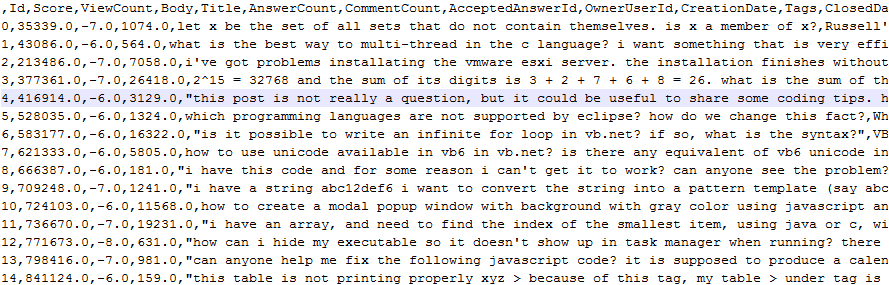
\includegraphics[width=0.8\textwidth]{tag_features_raw}
	\caption{Question without external tags detected.}
	\label{fig:tag_features_raw}
\end{figure}
\begin{figure}[ht]
	\centering
	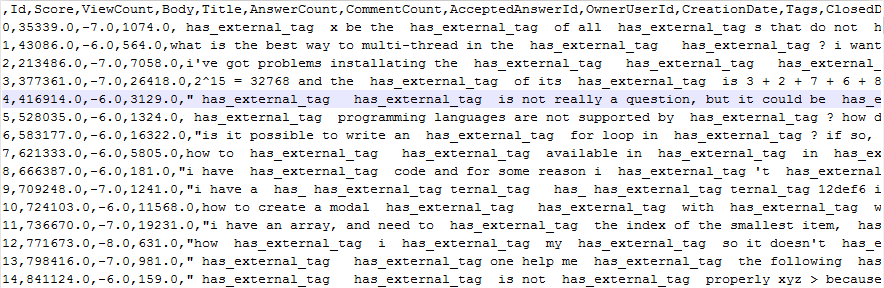
\includegraphics[width=0.8\textwidth]{tag_features_external}
	\caption{Question with external tags detected.}
	\label{fig:tag_features_external}
\end{figure}

\clearpage
\section{Scikit-learns roadmap - Choosing the right estimator}
\label{app:ml_map}
% image of the cheat-sheet from scikit-learn
\begin{figure}[ht]
	\centering
	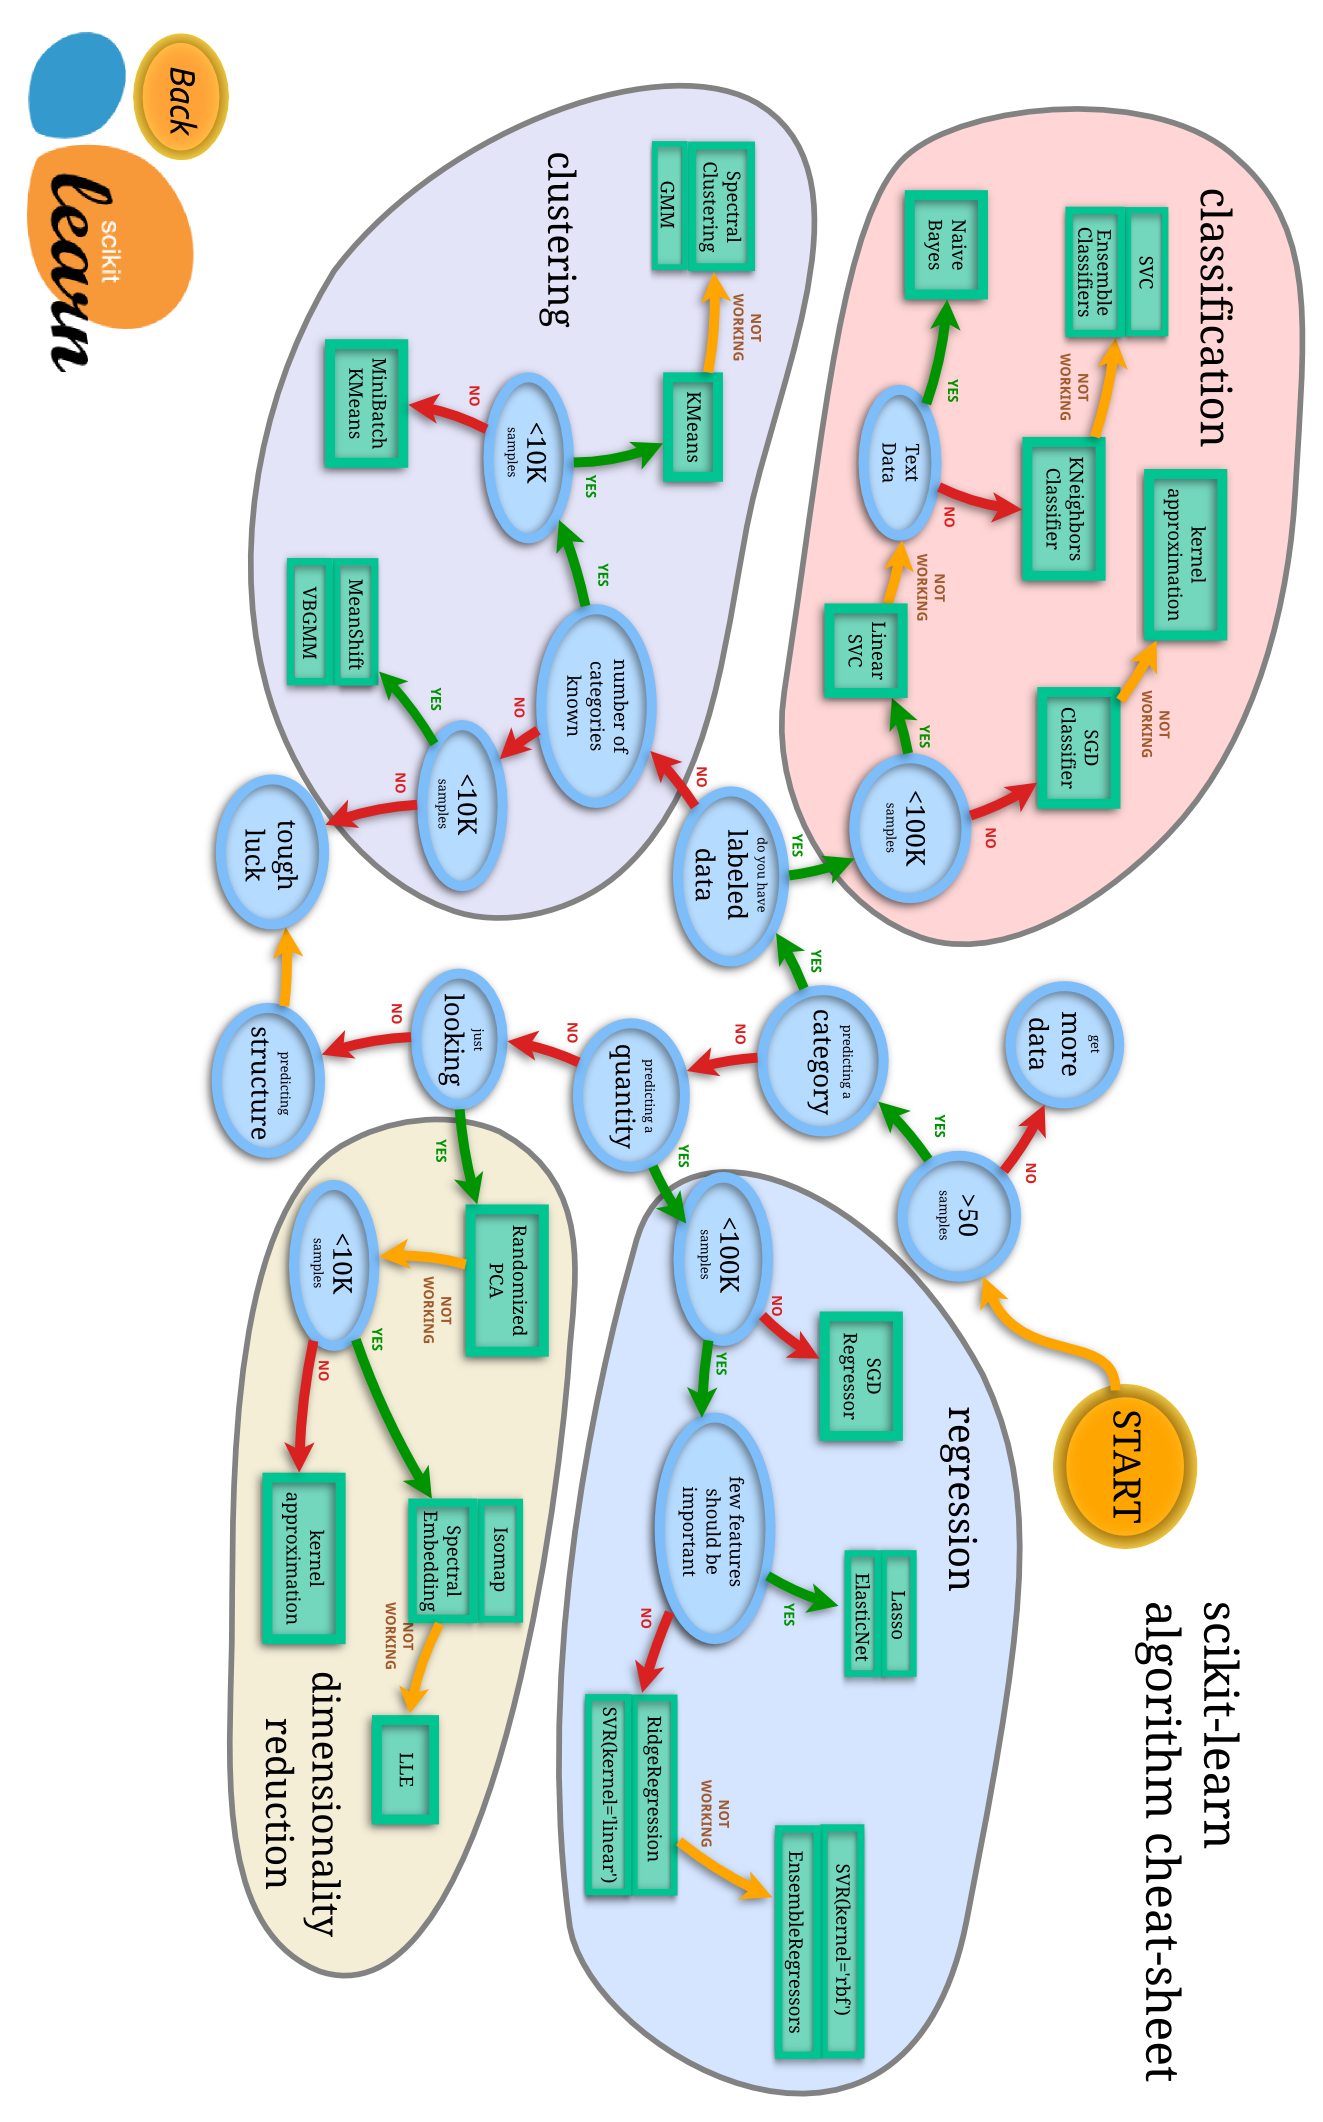
\includegraphics[width=0.645\textwidth]{ml_map}
	\caption[Choosing the right estimator]{Choosing the right estimator \cite{Scikitlearn.org2016i}.}
	\label{fig:ml_map}
\end{figure}

\clearpage
\section{Quick installation guide for Windows x64}
\label{app:installation_windows}
Since Python is much more adapted to *nix systems then Windows, I decided to write a short guide on how to install Python 3.5 and Scikit-learn on Windows. 
This guide is provided as-is, and I make no guarantees that this will result in a functioning installation, but it should at least reduce the problems. 
A presumption here is that the operative system is Windows x64 (if you have x86, you can ignore all the x64 settings).
Before installing anything, download the following:
\begin{itemize}
	\item Python: \url{https://www.python.org/downloads/windows/}. \\
	Select the Python version with "Windows x86-64" in its name.
	\item CygWin: \url{https://cygwin.com/}
	\item MinGW: \url{http://www.mingw.org/}
	\item MySQL connector for Python (Git; only needed for running this project): \\
	\url{https://github.com/mysql/mysql-connector-python}.
	\item x64 version of Numpy and Scipy \cite{Codementor.io2015,Gehrcke2015}: \\ 
	\url{http://www.lfd.uci.edu/~gohlke/pythonlibs/}. \\ 
	The latest available versions at the time of writing is "\emph{numpy-1.11.1rc1+mkl-cp35-cp35m-win\_amd64.whl}" and "\emph{scipy-0.17.1-cp35-cp35m-win\_amd64.whl}".
	\item Scikit-learn (Git): \url{https://github.com/scikit-learn/scikit-learn}
	\item If you do not have a version of Microsoft Visual Studio installed, you need to install Visual Studio 2013 or newer (because compiler requires it)\footnote{
		"vcvarsall.bat needed for python to compile missing from visual studio 2015": \\
		\url{http://stackoverflow.com/q/33323172}
	}.
\end{itemize}
% editor space
\begin{enumerate}
	\item Install Python, update pip, and install these packages: \\
	\emph{pip install -U bs4 pandas nltk matplotlib cython nose nosetests}
	\item Install MinGW.
	 Thereafter select "mingw32-base" under "MinGW Base System".
	In addition, under "MinGW Base System", select all belonging to Class "bin" and "dll"
	\item Install CygWin. 
	During installation, you will be asked what you want to install. 
	Select all entries that contains "gcc", "mingw64", "make", "automake", "lapack" and "openblas".
	The GCC-compilers are used in combination with MinGW, because Scikit-learn needs Fortran, Lapack and OpenBlas for \emph{make} to succeed.
	\item Change to folder with the x64 version of Numpy and Scipy, and install them~\cite{Codementor.io2015,Gehrcke2015}: \\
	\emph{pip install "numpy-1.11.1rc1+mkl-cp35-cp35m-win\_amd64.whl"} \\
	Verify installation: 1. \emph{python}, 2. \emph{import numpy}, 3. \emph{numpy.\_\_version\_\_}. \\
	\emph{pip install "scipy-0.17.1-cp35-cp35m-win\_amd64.whl"} and verify using the same steps, swapping numpy with scipy.
	\item Start CygWin (run as administrator), change to directory containing Scikit-learn and run the following commands: \\
	\emph{python setup.py build}  and \emph{python setup.py install}.
	\item If you want to use \gls{nltk}, you need to run \emph{python}, \emph{import nltk} and \emph{ntlk.download()} to download the corpus.
\end{enumerate}


% backup of various created tables


\begin{comment}

td-10000-Unprocessed
--------------------
Confusion matrix for test set classification:
[[1591  403]
[ 401 1605]]
Accuracy score for test set:
0.799
Classification Report:
			Precision	Recall		F1-score	Support

-1       0.80      0.80      0.80      1994
1       0.80      0.80      0.80      2006

avg / total       0.80      0.80      0.80      4000


Creating singular feature detector:  Code blocks
-----------------------------------------------
Confusion matrix for test set classification:
[[1574  420]
[ 413 1593]]
Accuracy score for test set:
0.79175
Classification Report:
			Precision	Recall		F1-score	Support

-1       0.79      0.79      0.79      1994
1       0.79      0.79      0.79      2006

avg / total       0.79      0.79      0.79      4000


Creating singular feature detector:  Links
-------------------------------------------
Confusion matrix for test set classification:
[[1584  410]
[ 416 1590]]
Accuracy score for test set:
0.7935
Classification Report:
			Precision	Recall		F1-score	Support

-1       0.79      0.79      0.79      1994
1       0.80      0.79      0.79      2006

avg / total       0.79      0.79      0.79      4000


Creating singular feature detector:  Homework
----------------------------------------
Confusion matrix for test set classification:
[[1590  404]
[ 400 1606]]
Accuracy score for test set:
0.799
Classification Report:
			Precision	Recall		F1-score	Support

-1       0.80      0.80      0.80      1994
1       0.80      0.80      0.80      2006

avg / total       0.80      0.80      0.80      4000


Creating singular feature detector:  Numerical
----------------------------------------
Confusion matrix for test set classification:
[[1591  403]
[ 375 1631]]
Accuracy score for test set:
0.8055
Classification Report:
			Precision	Recall		F1-score	Support

-1       0.81      0.80      0.80      1994
1       0.80      0.81      0.81      2006

avg / total       0.81      0.81      0.81      4000


Creating singular feature detector:  Hexadecimal
----------------------------------------
Confusion matrix for test set classification:
[[1591  403]
[ 401 1605]]
Accuracy score for test set:
0.799
Classification Report:
			Precision	Recall		F1-score	Support

-1       0.80      0.80      0.80      1994
1       0.80      0.80      0.80      2006

avg / total       0.80      0.80      0.80      4000


Creating singular feature detector:  Tags
----------------------------------------
Confusion matrix for test set classification:
[[1508  486]
[ 467 1539]]
Accuracy score for test set:
0.76175
Classification Report:
			Precision	Recall		F1-score	Support

-1       0.76      0.76      0.76      1994
1       0.76      0.77      0.76      2006

avg / total       0.76      0.76      0.76      4000


All features using 10k-unprocessed settings
----------------------------------------
Confusion matrix for test set classification:
[[1558  436]
[ 401 1605]]
Accuracy score for test set:
0.79075
Classification Report:
			Precision	Recall		F1-score	Support

-1       0.80      0.78      0.79      1994
1       0.79      0.80      0.79      2006

avg / total       0.79      0.79      0.79      4000


Creating model without stemming, using exhaustive search
------------------------------------------------------------
Confusion matrix for test set classification:
[[1567  427]
[ 408 1598]]
Accuracy score for test set:
0.79125
Classification Report:
			Precision	Recall		F1-score	Support

-1       0.79      0.79      0.79      1994
1       0.79      0.80      0.79      2006

avg / total       0.79      0.79      0.79      4000


td-10k
----------------------------------------
Confusion matrix for test set classification:
[[1558  436]
[ 525 1481]]
Accuracy score for test set:
0.75975
Classification Report:
			Precision	Recall		F1-score	Support

-1       0.75      0.78      0.76      1994
1       0.77      0.74      0.76      2006

avg / total       0.76      0.76      0.76      4000


td-10k-no-stemming
---------------------------------------------
Confusion matrix for test set classification:
[[1568  426]
[ 408 1598]]
Accuracy score for test set:
0.7915
Classification Report:
			Precision	Recall		F1-score	Support

-1       0.79      0.79      0.79      1994
1       0.79      0.80      0.79      2006

avg / total       0.79      0.79      0.79      4000


10k-sgd-loss-log
----------------------------------------
Confusion matrix for test set classification:
[[1610  384]
[ 594 1412]]
Accuracy score for test set:
0.7555
Classification Report:
			Precision	Recall		F1-score	Support

-1       0.73      0.81      0.77      1994
1       0.79      0.70      0.74      2006

avg / total       0.76      0.76      0.75      4000


10k-unprocessed-sgd
------------------
Confusion matrix for test set classification:
[[1607  387]
[ 418 1588]]
Accuracy score for test set:
0.79875
Classification Report:
			Precision	Recall		F1-score	Support

-1       0.79      0.81      0.80      1994
1       0.80      0.79      0.80      2006

avg / total       0.80      0.80      0.80      4000


10k-unprocessed-sgd-log-loss
------------------
Confusion matrix for test set classification:
[[1607  387]
[ 418 1588]]
Accuracy score for test set:
0.79875
Classification Report:
			Precision	Recall		F1-score	Support

-1       0.79      0.81      0.80      1994
1       0.80      0.79      0.80      2006

avg / total       0.80      0.80      0.80      4000


td-10k-all-features-occurrence-only
------------------
Confusion matrix for test set classification:
[[1268  403]
[ 329 1512]]
Accuracy score for test set:
0.791571753986
Classification Report:
			Precision	Recall		F1-score	Support

-1.0       0.79      0.76      0.78      1671
1.0       0.79      0.82      0.81      1841

avg / total       0.79      0.79      0.79      3512


td-10l-unprocessed-codeblocks
------------------------------------
Confusion matrix for test set classification:
[[793 195]
[218 765]]
Accuracy score for test set:
0.790461694571
Classification Report:
			Precision	Recall		F1-score	Support

-1.0       0.78      0.80      0.79       988
1.0       0.80      0.78      0.79       983

avg / total       0.79      0.79      0.79      1971


td-10l-unprocessed-hexadecimal
------------------------------------
Confusion matrix for test set classification:
[[21  0]
[ 6  5]]
Accuracy score for test set:
0.8125
Classification Report:
			Precision	Recall		F1-score	Support

-1.0       0.78      1.00      0.88        21
1.0       1.00      0.45      0.62        11

avg / total       0.85      0.81      0.79        32


td-10l-unprocessed-homework
------------------------------------
Confusion matrix for test set classification:
[[50  6]
[ 7 12]]
Accuracy score for test set:
0.826666666667
Classification Report:
			Precision	Recall		F1-score	Support

-1.0       0.88      0.89      0.88        56
1.0       0.67      0.63      0.65        19

avg / total       0.82      0.83      0.83        75


td-10l-unprocessed-links
------------------------------------
Confusion matrix for test set classification:
[[ 87  64]
[ 30 335]]
Accuracy score for test set:
0.817829457364
Classification Report:
			Precision	Recall		F1-score	Support

-1.0       0.74      0.58      0.65       151
1.0       0.84      0.92      0.88       365

avg / total       0.81      0.82      0.81       516


td-10l-unprocessed-numeric
------------------------------------
Confusion matrix for test set classification:
[[1043  111]
[ 256  395]]
Accuracy score for test set:
0.796675900277
Classification Report:
			Precision	Recall		F1-score	Support

-1.0       0.80      0.90      0.85      1154
1.0       0.78      0.61      0.68       651

avg / total       0.79      0.80      0.79      1805


td-10l-unprocessed-tags
------------------------------------
Confusion matrix for test set classification:
[[1487  498]
[ 442 1567]]
Accuracy score for test set:
0.764646970456
Classification Report:
			Precision	Recall		F1-score	Support

-1.0       0.77      0.75      0.76      1985
1.0       0.76      0.78      0.77      2009

avg / total       0.76      0.76      0.76      3994

td-10l-unprocessed-all-features
------------------------------------
Confusion matrix for test set classification:
[[1284  387]
[ 342 1499]]
Accuracy score for test set:
0.792425968109
Classification Report:
			Precision	Recall		F1-score	Support

-1.0       0.79      0.77      0.78      1671
1.0       0.79      0.81      0.80      1841

avg / total       0.79      0.79      0.79      3512


td-10l-unprocessed-up-codeblocks
------------------------------------
Confusion matrix for test set classification:
[[786 202]
[215 768]]
Accuracy score for test set:
0.788432267884
Classification Report:
			Precision	Recall		F1-score	Support

-1.0       0.79      0.80      0.79       988
1.0       0.79      0.78      0.79       983

avg / total       0.79      0.79      0.79      1971


td-10l-unprocessed-up-hex
------------------------------------
Confusion matrix for test set classification:
[[21  0]
[ 6  5]]
Accuracy score for test set:
0.8125
Classification Report:
			Precision	Recall		F1-score	Support

-1.0       0.78      1.00      0.88        21
1.0       1.00      0.45      0.62        11

avg / total       0.85      0.81      0.79        32


td-10l-unprocessed-up-homework
------------------------------------
Confusion matrix for test set classification:
[[52  4]
[ 8 11]]
Accuracy score for test set:
0.84
Classification Report:
					precision    	recall  	f1-score   	support

-1.0       			0.87      		0.93      	0.90        56
1.0       			0.73      		0.58      	0.65        19

avg / total       	0.83     	 	0.84      	0.83        75


td-10l-unprocessed-up-links
------------------------------------
Confusion matrix for test set classification:
[[ 95  56]
[ 28 337]]
Accuracy score for test set:
0.837209302326
Classification Report:
			Precision	Recall		F1-score	Support

-1.0       0.77      0.63      0.69       151
1.0       0.86      0.92      0.89       365

avg / total       0.83      0.84      0.83       516


td-10l-unprocessed-up-numeric
------------------------------------
Confusion matrix for test set classification:
[[1044  110]
[ 247  404]]
Accuracy score for test set:
0.802216066482
Classification Report:
			Precision	Recall		F1-score	Support

-1.0       0.81      0.90      0.85      1154
1.0       0.79      0.62      0.69       651

avg / total       0.80      0.80      0.80      1805


td-10l-unprocessed-up-tags
------------------------------------
Confusion matrix for test set classification:
[[1559  426]
[ 398 1611]]
Accuracy score for test set:
0.793690535804
Classification Report:
			Precision	Recall		F1-score	Support

-1.0       0.80      0.79      0.79      1985
1.0       0.79      0.80      0.80      2009

avg / total       0.79      0.79      0.79      3994

\end{comment}


\begin{comment}
\begin{table}[!htb]
\caption{Confusion Matrix for xxxxx.}
\begin{minipage}{.5\linewidth}
\caption{Unprocessed dataset}
\centering
\begin{tabular}{| c | c | c |}
\hline
Actual 		& Predicted: -1	& Predicted: 1	\\ \hline
-1			& xx			& xx			\\ \hline
1			& xx			& xx			\\ \hline
\end{tabular}
\end{minipage}%
\begin{minipage}{.5\linewidth}
\centering
\caption{All features}
\begin{tabular}{| c | c | c |}
\hline
Actual 		& Predicted: -1	& Predicted: 1	\\ \hline
-1			& xx			& xx			\\ \hline
1			& xx			& xx			\\ \hline
\end{tabular}
\end{minipage} 
\end{table}	
\end{comment}
\begin{comment}
% potentially flip this, and this as a Score X feature (since all kernel values were the same)
% something like "Comparison ..., with Kernel = RBF, Gamma = gamma and C = c
% and the table having features as rows, and score X unprocessed as column
\begin{table}[tbp]
\centering
\begin{tabular}{| c | c | c | c | c | c | c | c |}
\hline
~ 					& Code block	& Numerical		& Hexadecimal	& Homework		& Link 		& Tags	\\ \hline
Score 				& 0.783			& 0.796			& 0.793			& 0.794			& 0.795 	& 0.757	\\ \hline
C					& 1000			& 1000			& 1000			& 1000			& 1000 		& 1000	\\ \hline
Gamma ($\gamma$)	& 0.001			& 0.001			& 0.001			& 0.001			& 0.001 	& 0.001	\\ \hline
Kernel				& RBF			& RBF			& RBF			& RBF			& RBF 		& RBF	\\ \hline
\end{tabular}
\caption{Comparison of raw data set (unprocessed) and singular feature detectors}
%\label{tab:singular_feature_detector_so2}
\end{table}

\begin{table}[tbp]
\centering
\begin{tabular}{| c | c | c | c | c |}
\hline
~				& Votes < 0			& Votes = 0			& Votes > 0		& All			\\ \hline
Amount			& 659,955			& 5,256,105			& 5,286,971		& 11,203,031	\\ \hline
Oldest			& 06.08.2008		& 06.08.2008		& 31.07.2008	& 31.07.2008 	\\ \hline
Newest			& 06.03.2016		& 06.03.2016		& 06.03.2016	& 06.03.2016	\\ \hline
Vote (lowest)	& -147				& 0					& 1				& -147	 		\\ \hline
Vote (highest)	& -1				& 0					& 13845			& 13845	 		\\ \hline
\end{tabular}
\caption{Overview of the Stack Overflow dataset.}
%\label{tab:dataset_overview_so2}
\end{table}

Amount of features before anything was done to the text: 69766 - CountVectorizer(analyzer='word') - \%
Amount of features after adding stop word (English): 69462 - CountVectorizer(analyzer='word', stop\_words="english") - \%
Amount of features after removing code block, hexadecimals and numeric values: 27624 - \%
Amount of features after setting minimum document frequency: 440 - CountVectorizer(analyzer='word', min\_df=0.01, stop_words='english') - \%


Originally tagged questions as good/bad, but then switched to +/-1 due to considering switching to LibSVM.
\end{comment}

\end{document}
